\documentclass{iopart}
\usepackage{iopams}
\usepackage{braket,amsmath,xcolor,graphicx,cite}
\usepackage[colorlinks,linkcolor={blue},citecolor={blue}]{hyperref}
\usepackage[margin=2cm]{geometry}
\bibliographystyle{unsrt}

\begin{document}

\title{Supplementary Materials for ``Kondo frustration via charge fluctuations: a route to Mott localisation"}

\author{Abhirup Mukherjee$^1$, N. S. Vidhyadhiraja$^2$, A. Taraphder$^3$ and Siddhartha Lal$^1$}
\eads{\mailto{am18ip014@iiserkol.ac.in}, \mailto{raja@jncasr.ac.in}, \mailto{arghya@phy.iitkgp.ernet.in}, \mailto{slal@iiserkol.ac.in}}
\address{$^1$Department of Physical Sciences, Indian Institute of Science Education and Research-Kolkata, W.B. 741246, India}
\address{$^2$Theoretical Sciences Unit, Jawaharlal Nehru Center for Advanced Scientific Research, Jakkur, Bengaluru 560064, India}
\address{$^3$Department of Physics, Indian Institute of Technology Kharagpur, Kharagpur 721302, India}

\section{The unitary renormalisation group method}

The non-trivial nature of the impurity problem arises from the fact that the many-particle correlation between the impurity spin and the conduction electrons induces a many-particle interaction among the conduction electron states.
This means that within the conduction band, the states at high and low energies get entangled with each other, leading to what is called UV-IR mixing.
One of the methods of obtaining the low-energy physics while taking into account the effect of the high energy degrees of freedom is the renormalisation group (RG) approach.
The specific variant of RG used in this work is the unitary renormalisation group (URG) method developed by some of us in Refs.~\cite{santanukagome,anirbanmott1,anirbanmott2,1dhubjhep,siddharthacpi,anirban_mott_ent,anirban_kondo}.
The URG proceeds by applying unitary transformations on the Hamiltonian in order to decouple the high-energy \(k-\)states, leading to a reduction in the effective bandwidth and changes in the couplings for the low-energy degrees of freedom in the process.
This leads to a sequence of renormalised Hamiltonians, and hence the coupling RG equations.
While this is similar in spirit to the Poor Man's scaling approach of Anderson as applied to the single channel Kondo model~\cite{anderson1970}, there are several differences between the methods that will be apparent when we describe the method in more detail below.

We start by defining a UV-IR scheme for the single-particle electronic states \(\vec k = (k_F + |\vec k|) \hat k\).
We label the single-particle \(\vec k-\)states in terms of their normal distance $\Lambda = |\vec k|$ from the Fermi surface (FS) and the orientation of the unit vectors $\hat{s} = \hat k$, where $\hat{s}=\frac{\nabla\epsilon_{\mathbf{k}}}{|\nabla\epsilon_{\mathbf{k}}|}|_{\epsilon_{\mathbf{k}}=E_{F}}$.
Each \(\hat s\) represents a direction that is normal to the FS.
Combining these two labels with the spin index \(\sigma=\uparrow,\downarrow\), each single-particle state can be uniquely labelled as $\ket{j,l} = \ket{(k_F + \Lambda_j) \hat s,\sigma}, l\equiv (\hat{s},\sigma)$.
The $\Lambda$'s are arranged as follows: $\Lambda_{N}>\Lambda_{N-1}>\ldots>0$, such that \(\Lambda_N\) is farthest from the Fermi surface and is hence the most energetic (UV) while \(\Lambda_0\) is closest to the Fermi surface and is least energetic (IR).
The URG proceeds by disentangling these states \(\Lambda_j\), starting from those near the UV and gradually scaling towards the IR.
This leads to the Hamiltonian flow equation~\cite{anirbanurg1}
\begin{eqnarray}
\centering
\label{urg_map}
H_{(j-1)}=U_{(j)}H_{(j)}U^{\dagger}_{(j)}~,
\end{eqnarray}
where the unitary operation $U_{(j)}$ is the unitary map at RG step $j$. 
$U_{(j)}$ disentangles all the electronic states 
$|\mathbf{k}_{\Lambda_{j}\hat{s}_{m}},\sigma\rangle$
on the isogeometric curve and has the form~\cite{anirbanmott1,anirbanurg1}
\begin{eqnarray}
\centering U_{(j)}=\prod_{l}U_{j,l}, U_{j,l}=\frac{1}{\sqrt{2}}\sum_l [1+\eta_{j,l}-\eta^{\dagger}_{j,l}]~,
\end{eqnarray}
where \(l\) sums over the states on the isoenergetic shell at distance \(\Lambda_j\), and $\eta_{j,l}$ are electron-hole transition operators following the algebra
\begin{eqnarray}
	\left\{\eta_{j,l},\eta_{j,l}^{\dagger}\right\} = 1~,~\left[\eta_{j,l},\eta_{j,l}^{\dagger}\right] = 2\hat n_{j,l} - 1~.
\end{eqnarray}
The transition operator can be expressed in terms of the off-diagonal part of the Hamiltonian, \(H^X_{j,l} = Tr_{j,l}(c^{\dagger}_{j,l}H_{j})c_{j,l} + \text{h.c.}\), and the diagonal part \(H^D_{j,l}\) (kinetic energy and self-energies):
\begin{eqnarray}
	\eta_{j,l}&=&Tr_{j,l}(c^{\dagger}_{j,l}H_{j,l})c_{j,l}\frac{1}{\hat{\omega}_{j,l}-Tr_{j,l}(H^{D}_{j,l}\hat{n}_{j,l})\hat{n}_{j,l}}~.~~\label{e-TransOp}
\end{eqnarray}
The off-diagonal operator \(Tr_{j,l}(c^{\dagger}_{j,l}H_{j,l})c_{j,l}\) in the numerator of \(\eta_{j,l}\) contains all possible scattering vertices that change the configuration of the Fock state \(\ket{j,l}\)~\cite{anirbanurg1}. The generic forms of $H^{D}_{j,l}$ and $H^{X}_{j,l}$ are as follows
\begin{eqnarray}
H^{D}_{j,l}=&\sum_{\Lambda\hat{s},\sigma}\epsilon^{j,l}\hat{n}_{\mathbf{k}_{\Lambda\hat{s}},\sigma}+\sum_{\alpha}\Gamma_{\alpha}^{4,(j,l)}\hat{n}_{\mathbf{k}\sigma}\hat{n}_{\mathbf{k}'\sigma'} +\sum_{\beta}\Gamma_{\beta}^{6,(j,l)}\hat{n}_{\mathbf{k}\sigma}\hat{n}_{\mathbf{k}'\sigma'}\hat{n}_{\mathbf{k}''\sigma''}+\ldots~,\nonumber \\
H^{X}_{j,l}=&\sum_{\alpha}\Gamma_{\alpha}^{2}c^{\dagger}_{\mathbf{k}\sigma}c_{\mathbf{k}'\sigma'}+\sum_{\beta}\Gamma_{\beta}^{4}c^{\dagger}_{\mathbf{k}\sigma}c^{\dagger}_{\mathbf{k}'\sigma'}c_{\mathbf{k}_{1}'\sigma_{1}'}c_{\mathbf{k}_{1}\sigma_{1}}+\ldots~.
\end{eqnarray}
The indices \(\alpha\) and \(\beta\) are strings that denote the quantum numbers of the incoming and outgoing electronic states at a particular interaction vertex \(\Gamma^n_{\alpha}\) or  \(\Gamma^m_{\beta}\). The operator $\hat{\omega}_{j,l}$ accounts for the quantum fluctuations arising from the non-commutation between different parts of the renormalised Hamiltonian and has the following form~\cite{anirbanurg1}
\begin{eqnarray}
\hat{\omega}_{j,l}&=&H^{D}_{j,l}+H^{X}_{j,l}-H^{X}_{j,l-1}~.\label{qfOp}
\end{eqnarray}
Upon disentangling electronic states $\hat{s},\sigma$ along a isogeometric curve at distance $\Lambda_{j}$, the following effective Hamiltonian $H_{j,l}$ is generated 
\begin{eqnarray}
H_{j,l}=\prod_{m=1}^{l}U_{j,m}H_{(j)}[\prod_{m=1}^{l}U_{j,m}]^{\dagger}~.
\end{eqnarray}

Accounting for only the leading tangential scattering processes, as well as other momentum transfer processes along the normal direction $\hat{s}$, the renormalised Hamiltonian \(H_{(j-1)}\) has the form~\cite{anirbanurg1}
\begin{eqnarray}
Tr_{j,(1,\ldots,2n_{j})}(H_{(j)})+\sum_{l=1}^{2n_{j}}\lbrace c^{\dagger}_{j,l}Tr_{j,l}(H_{(j)}c_{j,l}),\eta_{j,l}\rbrace\tau_{j,l}~.\label{HRG}
\end{eqnarray}
The RG fixed point is reached when the denominator in eq.~\eqref{e-TransOp} vanishes, at a certain energy scale \(\Lambda^*\).
The vanishing of the denominator can be shown to be concomitant with the vanishing of the off-diagonal component \(H^X\)~\cite{anirbanurg1}, and the fixed point value of the quantum fluctuation operator is equal to one of the eigenvalues of the Hamiltonian.
The fixed point Hamiltonian \(H^*\) consists of the renormalised, still-entangled degrees of freedom \(\Lambda_j\) that lie inside the window \(\Lambda^*\): \(\Lambda_j < \Lambda^*\), as well as the integrals of motion (IOMs) that were decoupled by the URG transformations along the way.
The IOMs have been stripped of any number fluctuations and are therefore diagonal in the basis of the number operators for each of the decoupled degrees of freedom.
\begin{eqnarray}
	H^* = \sum_{\Lambda_j < \Lambda^*} H^*(\Lambda_j) + \sum_{\Lambda_j > \Lambda^*}H_\text{IOMs}(\Lambda_j)~.
\end{eqnarray}
The effective Hamiltonian can be used to construct the corresponding thermal density matrix and hence the partition function at a temperature \(T\):
\begin{eqnarray}
Z^* = \mathrm{Tr}\left[ \hat{\rho}^*\right] = \mathrm{Tr}\left[ e^{-\beta \hat{H}^{*}}\right] = \mathrm{Tr}\left[ U^{\dagger} e^{-\beta \hat{H}^{*}} U\right] = \mathrm{Tr}\left[ e^{-\beta \hat{H}}\right] = Z
\label{partfunc}~,
\end{eqnarray}
where \(\beta = 1/k_B T\), \(U = \prod_{1}^{j^{*}}U_{(j)}\), $H$ is the bare Hamiltonian and $j^{*}$ is the RG step at which the IR stable fixed point is reached. The unitary transformations preserve the partition function along the RG flow.

\section{Derivation of renormalisation group equations for the extended-SIAM}

The Hamiltonian we are working with is the extended Anderson impurity model (described in Section III of the main manuscript):
\begin{eqnarray}
	\mathcal{H} = -\frac{1}{2}U \left(\hat n_{d \uparrow} - \hat n_{d \downarrow}\right)^2 + \sum_{\vec k,\sigma} \epsilon_{\vec k} \tau_{\vec k,\sigma} + J \vec{S}_d\cdot\vec{S}_0 + V\sum_\sigma \left( c^\dagger_{d\sigma}c_{0\sigma} + \text{h.c.}\right) - \frac{1}{2}U_b \left(\hat n_{0 \uparrow} - \hat n_{0 \downarrow}\right)^2~.\quad
\end{eqnarray}
The renormalisation in the Hamiltonian \(H_{(j)}\) at the \(j^\text{th}\) RG step, upon decoupling an electronic state \(q\beta\), is given by the expression:
\begin{eqnarray}
	\left(\Delta H_{(j)}\right)_{\vec q,\beta} = H_{(j-1)} - H_{(j)} = c^\dagger_{\vec q,\beta} T_{\vec q,\beta} \frac{1}{\omega_e - H_D} T^\dagger_{\vec q,\beta}c_{\vec q,\beta} + T^\dagger_{\vec q,\beta} c_{\vec q,\beta} \frac{1}{\omega_h - H_D} c^\dagger_{\vec q,\beta}T_{\vec q,\beta}~,
\end{eqnarray}
where \(\omega_{e,h}\) are the quantum fluctuation scales for the electron and hole scattering channels, \(H_D\) is the part of the Hamiltonian that is diagonal in \(k-\)space, and \(T_{\vec q,\beta} + T_{\vec q,\beta}^\dagger\) is the part of the Hamiltonian that does not commute with \(\hat n_{\vec q,\beta}\) (in short, it is the part that is off-diagonal with respect to a particular state \(\vec q,\beta\)). This off-diagonal part is made up of contributions from \(V,J\) and \(U_b\): \(T_{\vec q \uparrow} = \left[V c^\dagger_{d \uparrow}  + J \sum_{\vec k}S_d^+ c^\dagger_{\vec k \downarrow}  + U_b \sum_{\vec k_1,\vec k_2,\vec k_3}c^\dagger_{\vec k_1 \uparrow} c^\dagger_{\vec k_3 \downarrow} c_{\vec k_4 \downarrow}\right] c_{\vec q \uparrow}\),
while the diagonal part is given by \(H_D = \epsilon_{\vec q} \tau_{q\uparrow} + \frac{1}{4}J S_d^z\left(\hat n_{q \uparrow} - \hat n_{q \downarrow}\right) - \frac{1}{2}U_b \left(\tau_{q \uparrow} - \tau_{q \downarrow}\right)^2\). The contribution from \(U_b\) is obtained by taking the Hartree contributions corresponding to the states \(\ket{q\sigma}\) from the full interacting term in the Hamiltonian.
Note that we have ignored potential scattering terms in the off-diagonal part \(T_{\vec q\beta}\). In order to allow both spin-flip and charge transfer scattering processes, we start from initial states with \(\tau_{q \uparrow} = -\tau_{q \downarrow}\). As a result, the contribution to \(H_D\) from the kinetic energy is \(\epsilon_q \tau_{q \uparrow} = \left(\pm D\right)\times\left(\pm\frac{1}{2}\right) = D/2\), while the contribution from \(U_b\) is \(-\frac{1}{2}U_b\left(\pm\frac{1}{2} - \left( \mp\frac{1}{2} \right) \right)^2 = -U_b/2 \).

\subsection{Renormalisation of \(U_b\)}
\(U_b\) can renormalise only via itself. The relevant renormalisation term in the particle sector is
\begin{eqnarray}
	U_b^2 \sum_{q\beta}\sum_{k_1,k_2,k_3,\atop{k_1^\prime,k_2^\prime,k_3^\prime}} c^\dagger_{q\beta}c_{k_1\beta}c^\dagger_{k_3\overline\beta}c_{k_1^\prime\overline\beta}\frac{1}{\omega - H_D}c^\dagger_{k_2^\prime\overline\beta}c_{k_3^\prime\overline\beta}c^\dagger_{k_2\beta}c_{q\beta}~.
\end{eqnarray}
In order to renormalise \(U_b\), we need to contract one more pair of momenta. There are two choices. The first is by setting \(k_3 = k_3^\prime = q\). The two internal states, then, are \(q\beta\) and \(q\overline\beta\). As discussed above, the intermediate state energy is \(-U_b/4\). We therefore have
\begin{eqnarray}
	\frac{U_b^2 n_j}{\omega - D/2 + \frac{U_b}{2}}\sum_{\beta}\sum_{k_1,k_2,k_1^\prime,k_2^\prime} c_{k_1\beta}c_{k_1^\prime\overline\beta}c^\dagger_{k_2^\prime\overline\beta}c^\dagger_{k_2\beta} = \frac{U_b^2 n_j}{\omega - D/2 + \frac{U_b}{2}}\sum_{\beta}\sum_{k_1,k_2,k_1^\prime,k_2^\prime} c^\dagger_{k_2^\prime\overline\beta}c_{k_1^\prime\overline\beta}c^\dagger_{k_2\beta}c_{k_1\beta}~.
\end{eqnarray}
Another way to contract the momenta is by setting \(k_1^\prime = k_2^\prime = q\), which gives a renormalisation of
\begin{eqnarray}
	\frac{U_b^2 n_j}{\omega - D/2 + \frac{U_b}{2}}\sum_{\beta}\sum_{k_1,k_2,k_3,k_3^\prime} c_{k_1\beta}c^\dagger_{k_3 \overline\beta}c_{k_3\prime\overline\beta}c^\dagger_{k_2\beta} = -\frac{U_b^2 n_j}{\omega - D/2}\sum_{\beta}\sum_{k_1,k_2,k_3,k_3^\prime} c^\dagger_{k_3 \overline\beta}c_{k_3\prime\overline\beta}c^\dagger_{k_2\beta}c_{k_1\beta}~.
\end{eqnarray}
The two contributions cancel each other. The same cancellation happens in the hole sector as well.

\subsection{Renormalisation of the impurity correlation \(U\)}
The coupling \(U\) is renormalised by two kinds of vertices: \(V^2\) and \(J^2\). We will consider these processes one at a time. For convenience, we define \(\epsilon_d = -U/2\).

The renormalisation arising from the first kind of terms, in the particle sector, is
\begin{eqnarray}
	\sum_{q\beta}c^\dagger_{q\beta}c_{d\beta}\frac{V^2}{\omega - H_D}c^\dagger_{d\beta}c_{q\beta} &= \sum_{q\beta}V^2 \hat n_{q\beta} \left( 1 - \hat n_{d\beta} \right)\left( \frac{1-\hat n_{d \overline\beta }}{\omega_0 - E_0} + \frac{\hat n_{d \overline\beta}}{\omega_1 - E_1}\right) \nonumber\\
												      &= V^2 n_j\sum_{\beta}\left( 1 - \hat n_{d\beta} \right)\left( \frac{1-\hat n_{d \overline\beta }}{\omega_0 - E_0} + \frac{\hat n_{d \overline\beta}}{\omega_1 - E_1}\right)~.
\end{eqnarray}
\(q\) runs over the momentum states that are being decoupled at this RG step: \(|q| = \Lambda_j\). \(E_{1,0}\) are the diagonal parts of the Hamiltonian at \(\hat n_{d\overline \beta}=1,0\) respectively: \(E_1 = \frac{D}{2}\) and \(E_0 = \frac{D}{2} + \epsilon_d - \frac{J}{4}\). In order to relate \(\omega_0\) and \(\omega_1\) with the common fluctuation scale \(\omega\) for the conduction electrons, we will replace these quantum fluctuation scales with the current renormalised values of the single-particle self-energy for the initial state from which we started scattering. For \(\hat n_{d\overline\beta}=0\), there is no additional self-energy because the impurity does not have any spin: \(\omega_0 = \omega\). For \(\hat n_{d\overline\beta} = 1\), we have an additional self-energy of \(\epsilon_d\) arising from the correlation on the impurity: \(\omega_1 = \omega + \epsilon_d\).
Substituting the values of \(E_{0,1}\) and \(\omega_{0,1}\), we get
\begin{eqnarray}
	\label{ren_ed_Vp}
	V^2 n_j\sum_{\beta}\left( 1 - \hat n_{d\beta} \right)\left( \frac{1-\hat n_{d \overline\beta }}{\omega - \frac{D}{2} - \epsilon_d + \frac{J}{4}} + \frac{\hat n_{d \overline\beta}}{\omega - \frac{D}{2} + \epsilon_d}\right)~.
\end{eqnarray}
Performing a similar calculation for the hole sector gives the contribution:
\begin{eqnarray}
	\label{ren_ed_Vh}
	V^2 n_j\sum_{\beta}\hat n_{d\beta}\left( \frac{1-\hat n_{d \overline\beta }}{\omega - \frac{D}{2} + \epsilon_d} + \frac{\hat n_{d \overline\beta}}{\omega - \frac{D}{2} - \epsilon_d + \frac{J}{4}}\right)~.
\end{eqnarray}
We now come to the second class of terms: spin-spin. We first look at the particle sector:
\begin{eqnarray}
	\label{ren_ed_Jpp}
	\frac{J^2}{4}\sum_{q\beta}c^\dagger_{d\overline\beta}c_{d\beta}c^\dagger_{q\beta}c_{-q\overline\beta} \frac{1}{\omega - H_D}c^\dagger_{d\beta}c_{d\overline\beta}c^\dagger_{q\overline\beta}c_{q\beta} = \frac{J^2}{4} n_j\frac{1}{\omega - \frac{D}{2} + \frac{J}{4}} \sum_{\beta}\hat n_{d\overline\beta}\left( 1 - \hat n_{d\beta} \right)~.
\end{eqnarray}
The diagonal part in the denominator was simple to deduce in this case because the nature of the scattering requires the spins \(S_d^z\) and \(\frac{\beta}{2}\left(\hat n_{q\beta} - \hat n_{q \overline\beta}\right)\) to be anti-parallel. This ensures that the intermediate state has an energy of \(E = \frac{D}{2} + \epsilon_d - \frac{J}{4}\), and the quantum fluctuation scale is \(\omega^\prime = \omega + \epsilon_d\), such that \(\omega^\prime - E = \omega - \frac{D}{2} + \frac{J}{4}\). In the hole sector, we have
\begin{eqnarray}
	\label{ren_ed_Jph}
	\frac{J^2}{4} n_j\frac{1}{\omega - \frac{D}{2} + \frac{J}{4}} \sum_{\beta}\hat n_{d\beta}\left( 1 - \hat n_{d\overline\beta} \right)~.
\end{eqnarray}
From eqs.~\eqref{ren_ed_Vp}, \eqref{ren_ed_Vh}, \eqref{ren_ed_Jpp} and \eqref{ren_ed_Jph}, we write
\begin{eqnarray}
	\Delta U &= \Delta \epsilon_2 + \Delta \epsilon_0 - 2\Delta \epsilon_1 \nonumber\\
		 &= -\frac{4V^2 n_j}{\omega + \frac{U_b}{2} - \frac{D}{2} - U/2} + \frac{4V^2 n_j}{\omega + \frac{U_b}{2} - \frac{D}{2} + U/2 + \frac{J}{4}} - \frac{J^2n_j}{\omega + \frac{U_b}{2} - \frac{D}{2} + \frac{J}{4}}~,
\end{eqnarray}
where we have restored the contribution from \(U_b\) in the denominator.

\subsection{Renormalisation of the hybridisation \(V\)}
Renormalisation of \(V\) happens through two kinds of processes: \(VJ\) and \(VU_b\). Within the first kind, the scattering can be either via \(S_d^z\) or through \(S_d^\pm\). For the first kind, we have the following contribution in the particle sector:
\begin{eqnarray}
	\sum_{q\beta} Vc^\dagger_{q\beta} c_{d\beta} \frac{1}{\omega - H_D}\frac{1}{4}J \sum_{k} \left(\hat n_{d\beta} - \hat n_{d\overline\beta}\right) c^\dagger_{k\beta}c_{q\beta} \nonumber\\
	= \frac{1}{4}V J n_j \frac{1}{2}\left(\frac{1}{\omega^\prime_1 - E} + \frac{1}{\omega^\prime_2 - E}\right)\sum_{k\beta} \left(1 - \hat n_{d\overline\beta}\right) c_{d\beta}c^\dagger_{k\beta}~.
\end{eqnarray}
The transformation from \(\frac{1}{\omega - H_D}\) to \(\frac{1}{2}\left(\frac{1}{\omega^\prime_1 - E} + \frac{1}{\omega^\prime_2 - E}\right)\) is made so that we can account for both the initial state and the final state energies through the two fluctuation scales \(\omega^\prime_1\) and \(\omega_2^\prime\) respectively; we calculate the denominators for both the initial and final states and then take the mean of the two (hence the factor of half in front). This was not required previously because, in the earlier scattering processes, the impurity returned to its initial state at the end, at least in terms of \(\epsilon_d \left( \hat n_{d \uparrow} - \hat n_{d \downarrow} \right)^2 \), and so we had \(\omega_1^\prime = \omega_2^\prime = \omega^\prime\).
Substituting the energies and the \(\omega-\)scales, we get
\begin{eqnarray}
	-\left(\frac{\frac{n_j}{4}V J \frac{1}{2}}{\omega - \frac{D}{2} + \frac{J}{4}} + \frac{\frac{n_j}{4}V J \frac{1}{2}}{\omega - \frac{D}{2} - \epsilon_d + \frac{J}{4}}\right)\sum_{k\beta}\left(1 - \hat n_{d\overline\beta}\right) c^\dagger_{k\beta} c_{d\beta}~.
\end{eqnarray}
One can generate another such process by exchanging the single-particle process and the spin-exchange process:
\begin{eqnarray}
	\sum_{q\beta} \frac{1}{4}J \sum_{k} \left(\hat n_{d\beta} - \hat n_{d\overline\beta}\right) c^\dagger_{q\beta}c_{k\beta} \frac{1}{\omega - H_D} V c^\dagger_{d\beta} c_{q\beta}~.
\end{eqnarray}
This is simply the Hermitian conjugate of the previous contribution. Combining this with the previous then gives
\begin{eqnarray}
	-\frac{n_j}{8}V J \left(\frac{1}{\omega - \frac{D}{2} + \frac{J}{4}} + \frac{1}{\omega - \frac{D}{2} - \epsilon_d + \frac{J}{4}}\right) \sum_{k\beta}\left(1 - \hat n_{d\overline\beta}\right) \times\left(c^\dagger_{d\beta} c_{k\beta} + \text{h.c.}\right)~.
\end{eqnarray}
If we similarly calculate the contributions from the spin-exchange processes involving \(S_d^\pm\), we get
\begin{eqnarray}
	-\frac{1}{4}V J n_j \left(\frac{1}{\omega - \frac{D}{2} + \frac{J}{4}} + \frac{1}{\omega - \frac{D}{2} - \epsilon_d + \frac{J}{4}}\right) \sum_{k\beta} \left(1 - \hat n_{d\beta}\right)  \left(c^\dagger_{k\overline\beta} c_{d\overline\beta} + \text{h.c.}\right)~.
\end{eqnarray}
The contributions from the hole sector are obtained by making the transformation \(\hat n_{d\overline\beta} \to 1 - \hat n_{d\overline\beta}\) on the particle sector contributions. The total renormalisation to \(V\) from \(VJ\) processes are
\begin{eqnarray}
	-\frac{3n_j}{8}V J \left(\frac{1}{\omega +U_b/4 - \frac{D}{2} + \frac{J}{4}} + \frac{1}{\omega +U_b/4 - \frac{D}{2} + U/2 + \frac{J}{4}}\right)\sum_{k\beta}\left(c^\dagger_{d\beta} c_{k\beta} + \text{h.c.}\right)~.
\end{eqnarray}
The renormalisation in \(V\) from \(U_b\) arises through terms of \(V U_b\) and \(U_b V\) kind. The first term gives
\begin{eqnarray}
	-\sum_{k\beta} c^\dagger_{d\beta} c_{k\beta} &\left[\frac{\hat n_{d\overline\beta}}{2}\left(\frac{n_jU_b V}{\omega - \frac{D}{2} - \frac{U}{2} + \frac{U_b}{4}} + \frac{n_jU_b V}{\omega - \frac{D}{2} + \frac{U_b}{4}}\right) \right.\nonumber\\
						     &\left.+ \frac{1-\hat n_{d\overline\beta}}{2}\left(\frac{n_jU_b V}{\omega - \frac{D}{2} + \frac{U_b}{4} + \frac{U}{2} + \frac{J}{4}} + \frac{n_jU_b V}{\omega - \frac{D}{2} + \frac{U_b}{4} + \frac{J}{4}}\right)\right]~.
\end{eqnarray}
The second term is of the form \(\sum_{q\beta}\sum_{k}U_b V c^\dagger_{q\beta}c_{d\beta} \frac{1}{\omega - H_D} \hat n_{q\overline\beta} c^\dagger_{k\beta}c_{q\beta}\),
and this is just the Hermitian conjugate of the previous term, so these two terms together lead to
\begin{eqnarray}
	-n_jU_b V\sum_{k\beta} \left(c^\dagger_{d\beta} c_{k\beta} + \text{h.c.}\right)&\left[\frac{\hat n_{d\overline\beta}}{2}\left(\frac{1}{\omega - \frac{D}{2} - \frac{U}{2} + \frac{U_b}{4}} + \frac{1}{\omega - \frac{D}{2} + \frac{U_b}{4}}\right) \right.\nonumber\\
											     &\left. + \frac{1-\hat n_{d\overline\beta}}{2}\left(\frac{1}{\omega - \frac{D}{2} + \frac{U_b}{4} + \frac{U}{2} + \frac{J}{4}} +\frac{1}{\omega - \frac{D}{2} + \frac{U_b}{4} + \frac{J}{4}}\right)\right]~.
\end{eqnarray}
In the hole sector, we have
\begin{eqnarray}
	-n_jU_b V\sum_{k\beta} c^\dagger_{k\beta} \left[\frac{\hat n_{d\overline\beta}}{2}\left(\frac{1}{\omega_1 - E_1} + \frac{1}{\omega^\prime_1 - E_1}\right) + \frac{1-\hat n_{d\overline\beta}}{2}\left(\frac{1}{\omega_0 - E_0} + \frac{1}{\omega_0^\prime - E_0}\right)\right] c_{d\beta}~.
\end{eqnarray}
\(E_1 = D/2 - U_b/4 - U/2 - J/4,~ ~ ~ E_0 = D/2 - U_b/4 - K/4\). The fluctuation scales are \(\omega_1 = \omega = \omega_0^\prime,~ ~ ~ \omega_1^\prime = \omega - U/2 = \omega_0\). Substituting these gives
\begin{eqnarray}
	-\sum_{k\beta} c^\dagger_{d\beta} c_{k\beta} &\left[\frac{1 - \hat n_{d\overline\beta}}{2}\left(\frac{n_jU_b V}{\omega - \frac{D}{2} - \frac{U}{2} + \frac{U_b}{4}} + \frac{n_jU_b V}{\omega - \frac{D}{2} + \frac{U_b}{4}}\right) + \frac{\hat n_{d\overline\beta}}{2}\left(\frac{n_jU_b V}{\omega - \frac{D}{2} + \frac{U_b}{4} + \frac{U}{2} + \frac{J}{4}} \right. \right. \nonumber\\
						     &\left.\left.+ \frac{n_jU_b V}{\omega - \frac{D}{2} + \frac{U_b}{4} + \frac{J}{4}}\right)\right]~.
\end{eqnarray}
The other term, obtained by exchanging \(V\) and \(U_b\), gives the Hermitian conjugate, so the overall contribution from the hole sector is the same as the total contribution from the particle sector, but with \(\hat n_{d\overline\beta} \to 1 - \hat n_{d\overline\beta}\). Combining both the sectors, we get
\begin{eqnarray}
	-\sum_{k\beta} \left(c^\dagger_{d\beta} c_{k\beta} + \text{h.c.}\right) &\left[\left(\frac{n_jU_b V/2}{\omega - \frac{D}{2} - \frac{U}{2} + \frac{U_b}{4}} + \frac{n_jU_b V/2}{\omega - \frac{D}{2} + \frac{U_b}{4}}\right) + \left(\frac{n_jU_b V/2}{\omega - \frac{D}{2} + \frac{U_b}{4} + \frac{U}{2} + \frac{J}{4}} \right.\right.\nonumber\\
										&\left.\left.+ \frac{n_jU_b V/2}{\omega - \frac{D}{2} + \frac{U_b}{4} + \frac{J}{4}}\right)\right]~.
\end{eqnarray}

\subsection{Renormalisation of the spin-exchange coupling \(J\)}
The term \(J \vec{S_d}\cdot\vec{S}_0\) can be split into three parts: \(J^z S_d^z, \frac{1}{2}J^+ S_d^+ S_0^-\) and \(\frac{1}{2}J^- S_d^- S_0^+\). We will only calculate the renormalisation in \(J^+\), which will be equal to that of \(J^-,J^z\) due to spin-rotation symmetry. The terms that renormalise \(J^+\) are of the form \(S_d^+ S_d^z\) and \(S_d^z S_d^+\). In the particle sector, we have
\begin{eqnarray}
	-\sum_{q} \sum_{kk^\prime}\frac{1}{4}J^2 S_d^+ c^\dagger_{q\downarrow}c_{k^\prime \uparrow} \frac{1}{\omega - H_D}S_d^z c^\dagger_{k \downarrow}c_{q \downarrow} = n_j \frac{1}{4}J^2 \left(-\frac{1}{2}S_d^+\right) \sum_{kk^\prime}c^\dagger_{k \downarrow}c_{k^\prime \uparrow} \frac{1}{\omega + \frac{U_b}{2} - \frac{D}{2} + \frac{J}{4}}~,\nonumber\\
	\sum_{q} \sum_{kk^\prime} \frac{1}{4}J^2 S_d^z c^\dagger_{q \uparrow}c_{k^\prime \uparrow} \frac{1}{\omega - H_D} S_d^+ c^\dagger_{k\downarrow}c_{q \uparrow} = -n_j \frac{1}{4}J^2 \left(\frac{1}{2}S_d^+\right) \sum_{kk^\prime}c^\dagger_{k \downarrow}c_{k^\prime \uparrow} \frac{1}{\omega + \frac{U_b}{2} - \frac{D}{2} + \frac{J}{4}}~.\qquad
\end{eqnarray}
The denominator is determined using \(E = \frac{D}{2} + \epsilon_d - \frac{J}{4}\) and \(\omega^\prime = \omega + \epsilon_d\).
In the hole sector, we similarly have
\begin{eqnarray}
	\sum_{q} \sum_{kk^\prime}\frac{1}{4}J^2 S_d^+ c^\dagger_{k\downarrow}c_{q \uparrow} \frac{1}{\omega - H_D}S_d^z c^\dagger_{q \uparrow}c_{k^\prime \uparrow} = n_j \frac{1}{4}J^2 \left(-\frac{1}{2}S_d^+\right) \sum_{kk^\prime}c^\dagger_{k \downarrow}c_{k^\prime \uparrow} \frac{1}{\omega + \frac{U_b}{2} - \frac{D}{2} + \frac{J}{4}}~,\nonumber\\
	-\sum_{q} \sum_{kk^\prime} \frac{1}{4}J^2 S_d^z c^\dagger_{k \downarrow}c_{q \downarrow} \frac{1}{\omega - H_D} S_d^+ c^\dagger_{q\downarrow}c_{k^\prime \uparrow} = -n_j \frac{1}{4}J^2 \left(\frac{1}{2}S_d^+\right) \sum_{kk^\prime}c^\dagger_{k \downarrow}c_{k^\prime \uparrow} \frac{1}{\omega + \frac{U_b}{2} - \frac{D}{2} + \frac{J}{4}}~.
\end{eqnarray}
The renormalisation due to \(U_b\) also happens through multiple terms. One of the terms is
\begin{eqnarray}
	\frac{1}{2} J U_b \sum_{q} \sum_{k,k^\prime} S_d^+ c^\dagger_{q \downarrow} c_{k \uparrow} \frac{1}{\omega - H_D} \hat n_{q \uparrow} c^\dagger_{k^\prime \downarrow}c_{q \downarrow} = -\frac{1}{2}\frac{J U_b n_j}{\omega - \frac{D}{2} + \frac{U_b}{2} + \frac{J}{4}} \sum_{k,k^\prime} S_d^+ c^\dagger_{k^\prime \downarrow} c_{k \uparrow}~.
\end{eqnarray}
The factor of half in front is the same half factor that appears in front of the \(S_1^+ S_2^-, S_1^-S_2^+\) terms when we rewrite \(\vec{S}_1\cdot\vec{S}_2\) in terms of \(S^z, S^\pm\). Another term is obtained by switching \(J\) and \(U_b\):
\begin{eqnarray}
	\frac{1}{2} J U_b \sum_{q} \sum_{k,k^\prime} \hat n_{q \downarrow} c^\dagger_{q \uparrow} c_{k \uparrow} \frac{1}{\omega - H_D}S_d^+ c^\dagger_{k^\prime \downarrow} c_{q \uparrow} = -\frac{1}{2}\frac{J U_b n_j}{\omega - \frac{D}{2} + \frac{U_b}{2} + \frac{J}{4}} \sum_{k,k^\prime} S_d^+ c^\dagger_{k^\prime \downarrow} c_{k \uparrow}~.
\end{eqnarray}

The corresponding terms in the hole sector are
\begin{eqnarray}
	-\frac{1}{2}\frac{J U_b n_j}{\omega - \frac{D}{2} + \frac{U_b}{2} + \frac{J}{4}} \sum_{k,k^\prime} S_d^+ c^\dagger_{k^\prime \downarrow} c_{k \uparrow}~, -\frac{1}{2}\frac{J U_b n_j}{\omega - \frac{D}{2} + \frac{U_b}{2} + \frac{J}{4}} \sum_{k,k^\prime} S_d^+ c^\dagger_{k^\prime \downarrow} c_{k \uparrow}~.
\end{eqnarray}

\subsection{Final URG equations}
In summary, the renormalisation in the couplings takes the form:
\begin{eqnarray}
	\Delta U &= 4V^2 n_j\left(\frac{1}{d_1} - \frac{1}{d_0}\right) - n_j\frac{J^2}{d_2},\quad &\Delta V = -\frac{3n_j V}{8}\left[J\left(\frac{1}{d_2} + \frac{1}{d_1}\right) +  \frac{4U_b}{3}\sum_{i=1}^4 \frac{1}{d_i}\right],\nonumber \\
	\Delta J &= -\frac{n_j J\left(J + 4U_b\right)}{d_2}~,\quad &\Delta U_b = 0\label{rg-eqn}~,
\end{eqnarray}
where the denominators \(d_i\) are given by
\begin{eqnarray}\label{rg-eqtn1}
	d_0 = \omega - \frac{D}{2} + \frac{U_b}{2} - \frac{U}{2},~d_1 = \omega - \frac{D}{2} + \frac{U_b}{2} + \frac{U}{2} + \frac{J}{4}~,\\
	d_2 = \omega - \frac{D}{2} + \frac{U_b}{2} + \frac{J}{4}~,d_3 = \omega - \frac{D}{2} + \frac{U_b}{2}~.
\end{eqnarray}
For the sake of completeness, we present the RG equation for a charge isospin Kondo coupling $K$ between the impurity and the bath: 
\begin{eqnarray}
\Delta K = -\frac{n_j K\left(K + 4U_b\right)}{\omega - \frac{D}{2} + \frac{U_b}{2} + \frac{K}{4}}~.
\end{eqnarray}
Indeed, the RG equation for $K$ is observed to be identical in form to that for the spin Kondo coupling $J$, obtained through the transformation \(J \to K\). This indicates that charge fluctuations between the bath zeroth and first sites (that are incited by an attractive interaction $U_{b}$) lead to the RG irrelevance of $K (>0)$, and thereby a destabilisation of the charge Kondo effect similar to that presented in the main manuscript for $J$.

\section{Expressing correlation functions in terms of entanglement}
\label{general-ent}

We will first relate the impurity Greens function to the geometric entanglement. Given a ground state \(\ket{\Psi}_\text{gs}\) and a spectrum of energies \(\left\{ E_n \right\} \), the retarded impurity Greens function (in time domain) is defined as \(G_{d\sigma}(t) = -i\theta(t)\braket{\left\{c_{d\sigma}(t),c^\dagger_{d\sigma}\right\}}\). It can be given a spectral representation in terms of the eigenstates \(\left\{\ket{\Psi}_n\right\}\) of the e-SIAM:
\begin{eqnarray}
	\label{green_spectral}
	G_{d\sigma}(\omega) = \frac{1}{Z}\sum_n \left[ \frac{|\braket{\Psi_\text{gs} | c_{d\sigma} | \Psi_n}|^2}{\omega + E_\text{gs} - E_n} + \frac{|\braket{\Psi_n | c_{d\sigma} | \Psi_\text{gs}}|^2}{\omega - E_\text{gs} + E_n}\right] ~,
\end{eqnarray}
where \(Z \equiv \sum_n e^{-\beta E_n}\) is the partition function.
We will now insert a complete basis into the expression. The basis will be the set of eigenstates of the Hamiltonian  \(H = H_1 + H_2\), where \(H_1\) is the two-site \(J-U_b\) Hamiltonian formed by the impurity and zeroth sites, and \(H_2\) is a tight-binding Hamiltonian formed by the remaining sites. Since the Hamiltonians are decoupled, the eigenstates \(\ket{\Psi}_{m,n}\) will be direct product states formed by combining the eigenstates \(\ket{\phi}_m,\ket{\psi}_n\) of the individual Hamiltonians \(H_1\) and \(H_2\) respectively: \(\ket{\Phi}_{m,n} = \ket{\phi}_m\otimes\ket{\psi}_n\). Inserting this basis leads to the expression:
\begin{eqnarray}
	\label{summation}
	\ket{\Psi}_\text{gs} = \sum_{m,n} \ket{\Phi}_{m,n} \left(\bra{\phi_{m}}\otimes\bra{\psi_n}\right)\ket{\Psi_\text{gs}}~.
\end{eqnarray}
The ground state of \(H_1\) is the spin-singlet: \(\ket{\phi}_0 = \ket{\text{ss}}\). We denote the ground state of the tight-binding Hamiltonian \(H_2\) by \(\ket{\psi}_0\). Because of the highly renormalised couplings \(V\) and \(J\), the impurity site is almost maximally entangled with the zeroth site, such that the ground state \(\ket{\Psi}_\text{gs}\) in the \(r < 0.25\) regime can be thought of as a direct product of the two-site ground state, \(c\ket{\text{ss}} + \sqrt{1-c^2}\ket{\text{ct}}\), in direct product with the tight-binding ground state:
\begin{eqnarray}
	\ket{\Psi}_\text{gs} \simeq \left(c\ket{\text{ss}} + \sqrt{1-c^2}\ket{\text{ct}}\right)  \otimes \ket{\psi}_0 = \ket{\Phi}_\text{ss} + \ket{\Phi}_\text{ct}~,
\end{eqnarray}
where \(\ket{\Phi}_\text{ss(ct)} = \ket{\text{ss}\left( \text{ct} \right)}\otimes\ket{\psi}_0 \).
This suggests that not all terms in the summation of eq.~\eqref{summation} contribute; out of all \(\left\{ \ket{\psi}_n \right\} \), only the ground state \(n=0\) contributes, while only \(\ket{ss}\) and \(\ket{ct}\) contribute from the set \(\left\{ \ket{\phi}_m \right\} \). The summation then simplifies to
\begin{eqnarray}
	\label{gs-ss}
	\ket{\Psi}_\text{gs} = \ket{\Phi}_{ss}\braket{\text{ss}|\Psi^{(2)}_\text{gs}} + \ket{\Phi}_{ct}\braket{\text{ct}|\Psi^{(2)}_\text{gs}}~,
\end{eqnarray}
where \(\ket{\Psi^{(2)}_\text{gs}}\) is the two-site part of the ground state and can be obtained by starting with the full ground state \(\ket{\Psi}_\text{gs}\) and tracing over the other lattice sites of the system.

We assume that the global phases of the wavefunctions are real, and since the internal weights of the wavefunctions are real as well, the overlaps \(\braket{\text{ss}|\Psi^{(2)}_\text{gs}},\braket{\text{ct}|\Psi^{(2)}_\text{gs}}\) are also real. We can use these overlaps to define a geometric measure of entanglement~\cite{shimony1995degree,wei2003geometric,horodecki2009quantum}:
\begin{eqnarray}
	\varepsilon\left(\psi_1,\psi_2\right) = 1 - |\braket{\psi_1 | \psi_2}|^2~.
\end{eqnarray}
If \(\ket{\psi_1}\) is thought of as a separable state, then \(\ket{\psi_2}\) should be less entangled if its overlap with \(\ket{\psi_1}\) is large, which is indeed borne out by the definition.
The overlaps then become \(\braket{\text{ss}|\Psi^{(2)}_\text{gs}} = \sqrt{1 - \varepsilon\left(ss,\Psi^{(2)}_\text{gs}\right)}\), and similarly for the state \(\ket{\text{ct}}\). For brevity, we will use the notation \(\varepsilon_\text{ss} \equiv \varepsilon\left(ss,\Psi^{(2)}_\text{gs}\right), \varepsilon_\text{ct} \equiv \varepsilon\left(ct,\Psi^{(2)}_\text{gs}\right)\). The retarded impurity Greens function for spin \(\sigma\) can now be written in terms of these measures:
\begin{eqnarray}\label{greens_func_entng}
	G_{d\sigma}(\omega) = \frac{1}{Z}\sum_n &\left[\left(1 - \varepsilon_\text{ss} \right) \left(\frac{|\braket{\Phi_\text{ss} | c_{d\sigma} | \Psi_n}|^2}{\omega + E_\text{gs} - E_n} + \frac{|\braket{\Psi_n | c_{d\sigma} | \Phi_\text{ss}}|^2}{\omega - E_\text{gs} + E_n}\right) + \left(1 - \varepsilon_\text{ct} \right) \frac{|\braket{\Phi_\text{ct} | c_{d\sigma} | \Psi_n}|^2}{\omega + E_\text{gs} - E_n}\right.\nonumber\\
		&\left. + \left(1 - \varepsilon_\text{ct} \right)\frac{|\braket{\Psi_n | c_{d\sigma} | \Phi_\text{ct}}|^2}{\omega - E_\text{gs} + E_n} + \sqrt{\left(1 - \varepsilon_\text{ss} \right)}\sqrt{\left(1 - \varepsilon_\text{ct} \right)} \frac{\braket{\Phi_\text{ss} | c_{d\sigma} | \Psi_n}\braket{\Psi_n | c^\dagger_{d\sigma} | \Phi_\text{ct}} + \text{h.c.}}{\omega + E_\text{gs} - E_n} \right. \nonumber\\
		&\left.+ \sqrt{\left(1 - \varepsilon_\text{ss} \right)}\sqrt{\left(1 - \varepsilon_\text{ct} \right)}\frac{\braket{\Phi_\text{ct} | c_{d\sigma} | \Psi_n}\braket{\Psi_n | c^\dagger_{d\sigma} | \Phi_\text{ss}} + \text{h.c.}}{\omega - E_\text{gs} + E_n}\right]~.
\end{eqnarray}

We now generalise this to any real-space two-particle correlation involving operators \(O_1, O_2\) that are at most two-particle operators and act on the combined Hilbert space of the impurity site and the zeroth site. The so-called lesser Greens function corresponding to these operators is defined as 
\begin{eqnarray}\label{lesser-gf}
	G^<_{O_1^\dagger, O_2}(t) \equiv i\braket{O_1^\dagger O_2(t)}, \quad G^<_{O_1^\dagger, O_2}(t\to \infty) = i\braket{\Psi_\text{gs}|O_1^\dagger O_2 | \Psi_\text{gs}} ~.
\end{eqnarray}
We focus on the static case (\(t \to \infty\)) here. Following eq.~\eqref{gs-ss}, we can rewrite the ground states in terms of the entanglement measures mentioned above.
\begin{eqnarray}
	\ket{\Psi}_\text{gs} = \ket{\Phi}_{ss}\sqrt{1 - \varepsilon_\text{ss}} + \ket{\Phi}_{ct}\sqrt{1 - \varepsilon_\text{ss}}~,
\end{eqnarray}
where \(\ket{\Phi}_\text{ss(ct)}\) are the zero spin and zero charge isospin eigenstates of the Hamiltonian \(H = H_1 + H_2\) defined below eq.~\eqref{green_spectral}.
Substituting this in the static lesser Greens function gives
\begin{eqnarray}
	\label{gen-entng}
	\frac{1}{i}G^<_{O_1^\dagger, O_2}(t\to \infty) =& \left(1 - \varepsilon_\text{ss}\right) \braket{\Phi_\text{ss} | O_2 O_1^\dagger | \Phi_\text{ss}} + \left(1 - \varepsilon_\text{ct}\right) \braket{\Phi_\text{ct} | O_2 O_1^\dagger | \Phi_\text{ct}} \nonumber \\
				      &+ \sqrt{1 - \varepsilon_\text{ss}}\sqrt{1 - \varepsilon_\text{ct}}\left(\braket{\Phi_\text{ss} | O_2 O_1^\dagger | \Phi_\text{ct}} + \braket{\Phi_\text{ct} | O_2 O_1^\dagger | \Phi_\text{s}}\right)~.
\end{eqnarray}
This can be extended to generalised retarded Greens functions \(G^R_{O_1^\dagger,O_2}(t) \equiv -i\theta(t) \braket{\left\{O_1^\dagger(t), O_2\right\}}\), whose spectral representation is of the form
\begin{eqnarray}
	\label{retarded}
	G^R_{O_1^\dagger,O_2}(\omega) = \frac{1}{Z}\sum_n \left[ \frac{\braket{\Psi_\text{gs} | O_2 | \Psi_n}\braket{\Psi_n | O_1^\dagger | \Psi_\text{gs}}}{\omega + E_\text{gs} - E_n} + \frac{\braket{\Psi_n | O_2 | \Psi_\text{gs}}\braket{\Psi_\text{gs} | O_1^\dagger | \Psi_n}}{\omega - E_\text{gs} + E_n}\right] ~.
\end{eqnarray}
Following an approach very similar to the one that led to eq.~\eqref{greens_func_entng}, we can cast the generalised Greens function in terms of the geometric entanglement measures:
\begin{eqnarray}
	G^R_{O_1^\dagger,O_2}(\omega) = \frac{1}{Z}\sum_n &\left[\left(1 - \varepsilon_\text{ss} \right) \left(\frac{\left(O_1\right)_{\text{ss},n}^* \left( O_2 \right)_{\text{ss}, n}}{\omega + E_\text{gs} - E_n} + \frac{\left(O_1\right)_{n,\text{ss}}^* \left( O_2 \right)_{n,\text{ss}}}{\omega - E_\text{gs} + E_n}\right) + \left(1 - \varepsilon_\text{ct} \right) \frac{\left(O_1\right)_{\text{ct},n}^* \left( O_2 \right)_{\text{ct}, n}}{\omega + E_\text{gs} - E_n}\right.\nonumber\\
						&\left. + \left(1 - \varepsilon_\text{ct} \right)\frac{\left(O_1\right)_{n,\text{ct}}^* \left( O_2 \right)_{n,\text{ct}}}{\omega - E_\text{gs} + E_n} + \sqrt{\left(1 - \varepsilon_\text{ss} \right)}\sqrt{\left(1 - \varepsilon_\text{ct} \right)} \frac{\left(O_2\right)_{\text{ss},n} \left( O_1 \right)_{\text{ct},n}^* + \text{h.c.}}{\omega + E_\text{gs} - E_n} \right. \nonumber\\
		&\left.+ \sqrt{\left(1 - \varepsilon_\text{ss} \right)}\sqrt{\left(1 - \varepsilon_\text{ct} \right)}\frac{\left(O_2\right)_{\text{ct},n} \left( O_1 \right)_{\text{ss},n}^* + \text{h.c.}}{\omega - E_\text{gs} + E_n}\right]~,
\end{eqnarray}
where \(\left( O_2 \right)_{\text{ss},n} \) is the matrix element \(\braket{\Phi_\text{ss} | O_2 | \Psi_n}\), and similar definitions exist for \(\left( O_1 \right)_{\text{ss},n} \) and its \(\ket{\Phi_\text{ct}}\) counterparts.

Closely related to geometric entanglement is the quantum Fisher information (QFI) \(F_Q\)~\cite{braunstein1994statistical,Hauke2016}, which quantifies how sensitive a state \(\rho\) is to unitary transformations generated by an observable \(\hat O\).
For a pure state \(\rho = \ket{\psi}\bra{\psi}\), \(F_Q (\psi,\hat O)\) is defined in terms of the variance of the operator $\hat O$ (i.e., the connected correlation function):
\begin{eqnarray}
	F_Q(\psi,\hat O) = 4 \Delta (\hat O)^{2}= 4\left(\braket{\psi|\hat O^2|\psi} - \braket{\psi|\hat O|\psi}^2\right)~,
\end{eqnarray}
and it provides an upper bound on the precision that can be achieved in measuring the parameter \(\theta\) that is dual to the observable \(\hat O\): \(\mathcal{N}\left( \Delta \theta \right)^2 \geq F_Q^{-1} \), \(\mathcal{N}\) being the number of independent measurements~\cite{braunstein1994statistical,Hauke2016}. \(F_Q (\psi,\hat O)\) is thus a measure of the entanglement arising from quantum fluctuation content in $\ket{\psi}$ (considered with respect to an eigenstate of $\hat O$). This can be made more manifest by considering a traceless operator \(\hat M\) with eigenstates \(\left\{\ket{m}\right\}\). Without loss of generality, we can rescale the operator such that \(\sum m^2 = 1/2\). There are several examples of such operators in the context of the present work, such as the impurity magnetisation operator (\(S_d^z\)), the Kondo spin-flip operator (\(S_d^+ S_0^- + \text{h.c.}\)) and the Kondo isospin-flip operator (\(C_d^+ C_0^- + \text{h.c.}\)). If \(\varepsilon_m(\psi) \equiv 1 - |\braket{m | \psi}|^2\) is the geometric entanglement between a given state \(\ket{\psi}\) and the eigenstates of \(\hat M\), the QFI corresponding to \(\hat M\) in the state \(\psi\) can be written as
\begin{eqnarray}\label{QFI-geo-ent}
	F_Q(\psi,\hat M) = 4\left[\frac{1}{2} - \sum_m m^2\varepsilon_m - \left(\sum_m m\varepsilon_m\right)^2 \right] ~.
\end{eqnarray}
The total geometric entanglement \(\sum_m \varepsilon_m\) is constrained to be \(d_M - 1\), where \(d_M\) is the dimension of the operator \(\hat M\).
Because each eigenvalue \(m\) has a magnitude of at most \(1/\sqrt 2\) (all \(m^2\) must add up to \(1/2\)), the maximum magnitude of the last two terms in eq.~\eqref{QFI-geo-ent} (and hence the minimum value of the QFI) is attained for the case when some of the \(\varepsilon_m\) are zero.
However, because the eigenstates are orthogonal, only one of them can have perfect overlap with the state \(\ket{\psi}\) and only one \(\varepsilon_m\) can be zero at a time.
The case of minimum QFI therefore corresponds to \(\varepsilon_{m^*} = 0, \varepsilon_{m\neq m^*}=1\), leading to \(F_Q = 0\).
The opposite situation arises when all the geometric entanglement measures are non-zero and equal, \(\varepsilon_m = 1/d_M\), leading to a maximum QFI value of \(F_Q = 2/d_M\).
A uniformly spread geometric entanglement distribution, therefore, leads to a larger QFI, while a more focused distribution leads to a smaller QFI.
This sums up the relation between the quantum Fisher information and geometric entanglement.

If the operator \(\hat M\) is such that its eigenstates are separable states from the perspective of a certain party, the vanishing QFI arises when \(\ket{\psi}\) has zero geometric entanglement with respect to one of the separable states, and the QFI saturates when \(\ket{\psi}\) has a finite geometric entanglement with all of the states.
A large QFI can thus be associated with more entanglement. 
Moreover, if the eigenstates of \(\hat M\) are symmetry-broken states, a vanishing QFI indicates that \(\ket{\psi}\) is very close to such a symmetry-broken state, while a large QFI indicates that \(\ket{\psi}\) is a uniform superposition of such symmetry-broken states and therefore preserves the symmetry as a whole. A larger QFI points towards the presence of more quantum fluctuations and the lack of susceptibility towards symmetry-breaking.

In order to demonstrate these ideas in the present problem, we computed the QFI in the ground-state of the e-SIAM for a number of Hermitian operators, as a function of the parameter \(r=-U_b/J_0\).
These are shown in the left panel of Fig.~\eqref{QFI-esiam} (left panel). 
In order to explain the behaviour depicted in the figure, we point out again that the ground-states for \(r \ll r_{c2}\), \(r \lesssim r_{c2}\) and \(r > r_{c2}\) are \(\ket{\text{SS}} + \ket{\text{CT}}\), \(\ket{\text{SS}}\) and \(\ket{\text{LM}}\) respectively, where \(\ket{\text{SS}}\), \(\ket{\text{CT}}\) and $\ket{\text{LM}}$ are the spin-singlet state, charge triplet and local moment states respectively.
We focus on the spin-flip QFI, corresponding to the operator \(\hat O = S_d^+ S_0^- + \text{h.c.}\).
\begin{itemize}
	\item For \(r < r_{c1}\), the ground-state involves both \(\ket{SS}\) and \(\ket{CT}\), meaning that neither of the two entanglement measures \(\varepsilon_\text{SS}\) or \(\varepsilon_\text{CT}\) will be zero.
	As mentioned in the preceding paragraph, this leads to the maximal QFI, as can be seen in the figure as well.
	\item At \(r = r_{c1}\), the charge triplet content vanishes and the ground-state is purely a singlet beyond that point.
	As a result, in the range \(r_{c1} < r < r_{c2}\), the geometric entanglement corresponding to the singlet state is zero, leading to a minimal and vanishing QFI.
	This is again shown in the figure.
	\item Finally, for \(r > r_{c2}\), the local moment states become the ground-states, where the bath zeroth site displays all four configurations as a superposition, because of the hopping into the rest of the bath.
	This state is again not an eigenstate of the spin-flip operator, and the geometric entanglement will be uniformly distributed across the states, none being zero.
	This explains the large QFI in the local moment phase.
\end{itemize}
Similar explanations hold for the single-particle hopping FQI between the impurity and the zeroth site, and the charge isospin FQI between the zeroth site and the first site.
In Fig.~\eqref{QFI-esiam} (right panel), we show the QFI for the same three operators very close to the MIT (i.e., for $r\lesssim r_{c2}$). 
Two important quantities that track the local MIT and act as order parameters for the transition are the degree of compensation for the impurity (\(\braket{\vec{S}_d\cdot\vec{S}_0}\)) and the impurity magnetisation (\(\braket{S_d^z}\)), and the first two QFI (red and blue curves) in Fig.~\ref{QFI-esiam} are therefore particularly important because that they quantify the quantum fluctuations present in the system corresponding to these order parameters.
Our analysis shows that the two phases on either side of the transition are characterised by distinct values of this pair of QFI: while the QFI corresponding to the degree of compensation zero in the Kondo screened phase, it becomes non-zero in the local moment phase, and the opposite is true for the QFI arising from the impurity magnetisation.
The phase precisely at the transition is distinct from those on either side because it displays a non-zero value for both the QFI.
While it is expected that a critical point would show enhanced fluctuations of multiple kinds (giving rise to universality), it is enlightening to find that this is also reflected in a measure of many-particle entanglement.

All three QFIs are observed to saturate to finite, non-zero values at the MIT, indicating that the non-Fermi liquid state therein possesses quantum fluctuations of all three varieties. 

We will now relate the QFI to some other measures of correlation. The QFI corresponding to an observable can be directly related to the static lesser Greens functions associated with that observable:
\begin{eqnarray}
	\label{lesser-QFI}
	F_Q(\psi,\hat O_2) = 4\left(\braket{\hat O_2 \hat O_1^\dagger}\bigg|_{\hat O_1^\dagger=\hat O_2} - \braket{\hat O_2 \hat O_1^\dagger}^2\bigg|_{\hat O_1=1}\right) = 4\left[G^<_{O_2, O_2}(t\to \infty) - \left(G^<_{1, O_2}(t\to \infty)\right)^2\right]
\end{eqnarray}
In the context of the present work, eq.~\eqref{gen-entng} allows relating the QFI to the geometric entanglement measured with respect to the spin-singlet and charge triplet states. By combining eqs.~\eqref{gen-entng} and \eqref{lesser-QFI}, we get
\begin{eqnarray}
	F_Q(\psi,\hat O_2) &= 4\left[ \left(1 - \varepsilon_\text{ss}\right) \braket{\Phi_\text{ss} | \hat O_2^2 | \Phi_\text{ss}} + \left(1 - \varepsilon_\text{ct}\right) \braket{\Phi_\text{ct} | \hat O_2^2 | \Phi_\text{ct}} \right.\nonumber \\
			   &\left.+ \sqrt{1 - \varepsilon_\text{ss}}\sqrt{1 - \varepsilon_\text{ct}}\left(\braket{\Phi_\text{ss} | \hat O_2^2 | \Phi_\text{ct}} + \braket{\Phi_\text{ct} | \hat O_2^2 | \Phi_\text{s}}\right) - \left\{\left(1 - \varepsilon_\text{ss}\right) \braket{\Phi_\text{ss} | \hat O_2 | \Phi_\text{ss}} \right.\right.\nonumber\\
			   &\left.\left. + \left(1 - \varepsilon_\text{ct}\right) \braket{\Phi_\text{ct} | \hat O_2 | \Phi_\text{ct}} + \sqrt{1 - \varepsilon_\text{ss}}\sqrt{1 - \varepsilon_\text{ct}}\left(\braket{\Phi_\text{ss} | \hat O_2 | \Phi_\text{ct}} + \braket{\Phi_\text{ct} | \hat O_2 | \Phi_\text{s}}\right)\right\}^2 \right]~.
\end{eqnarray}
Further, the retarded Greens function defined above in eq.~\eqref{retarded} can very generally be related to the QFI.
By using the simplified forms \(\frac{i}{2}G^R_{O_2,O_2}(t \to \infty) = \braket{\left(O_2\right)^2}\) and \(\frac{i}{2}G^R_{1,O_2}(t \to \infty) = \braket{O_2}\), we get
\begin{eqnarray}
	F_Q(\psi,\hat O_2) = 2iG^R_{O_2, O_2}(t\to \infty) + \left(G^R_{1, O_2}(t\to \infty)\right)^2~.
\end{eqnarray}
\begin{figure}[htpb]
	\centering
	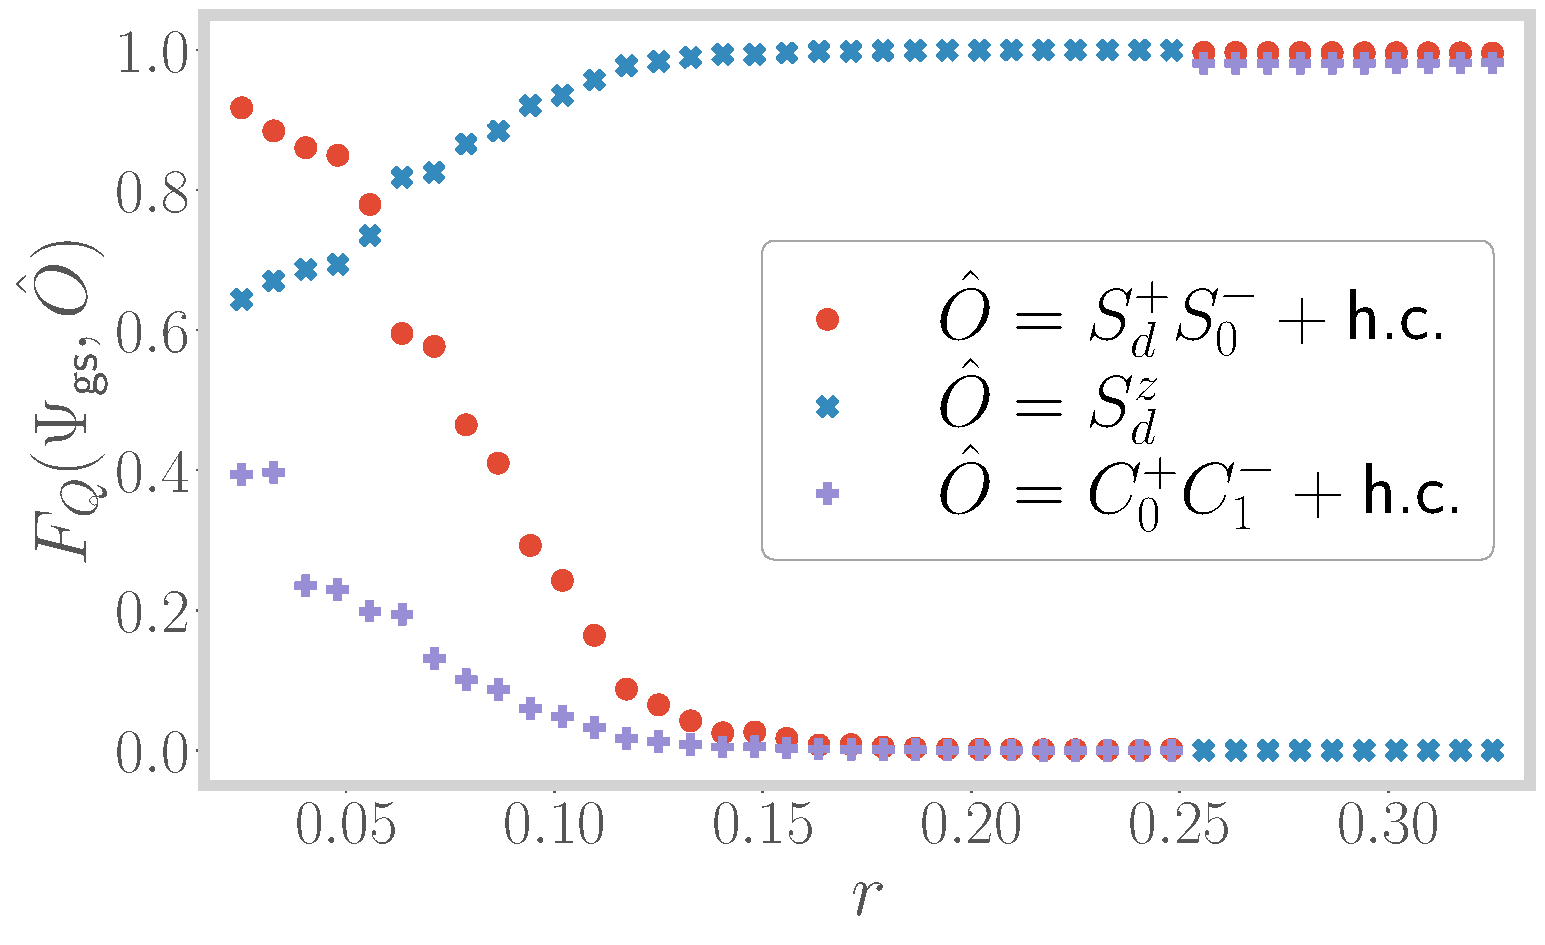
\includegraphics[width=0.48\textwidth]{QFI.pdf}
	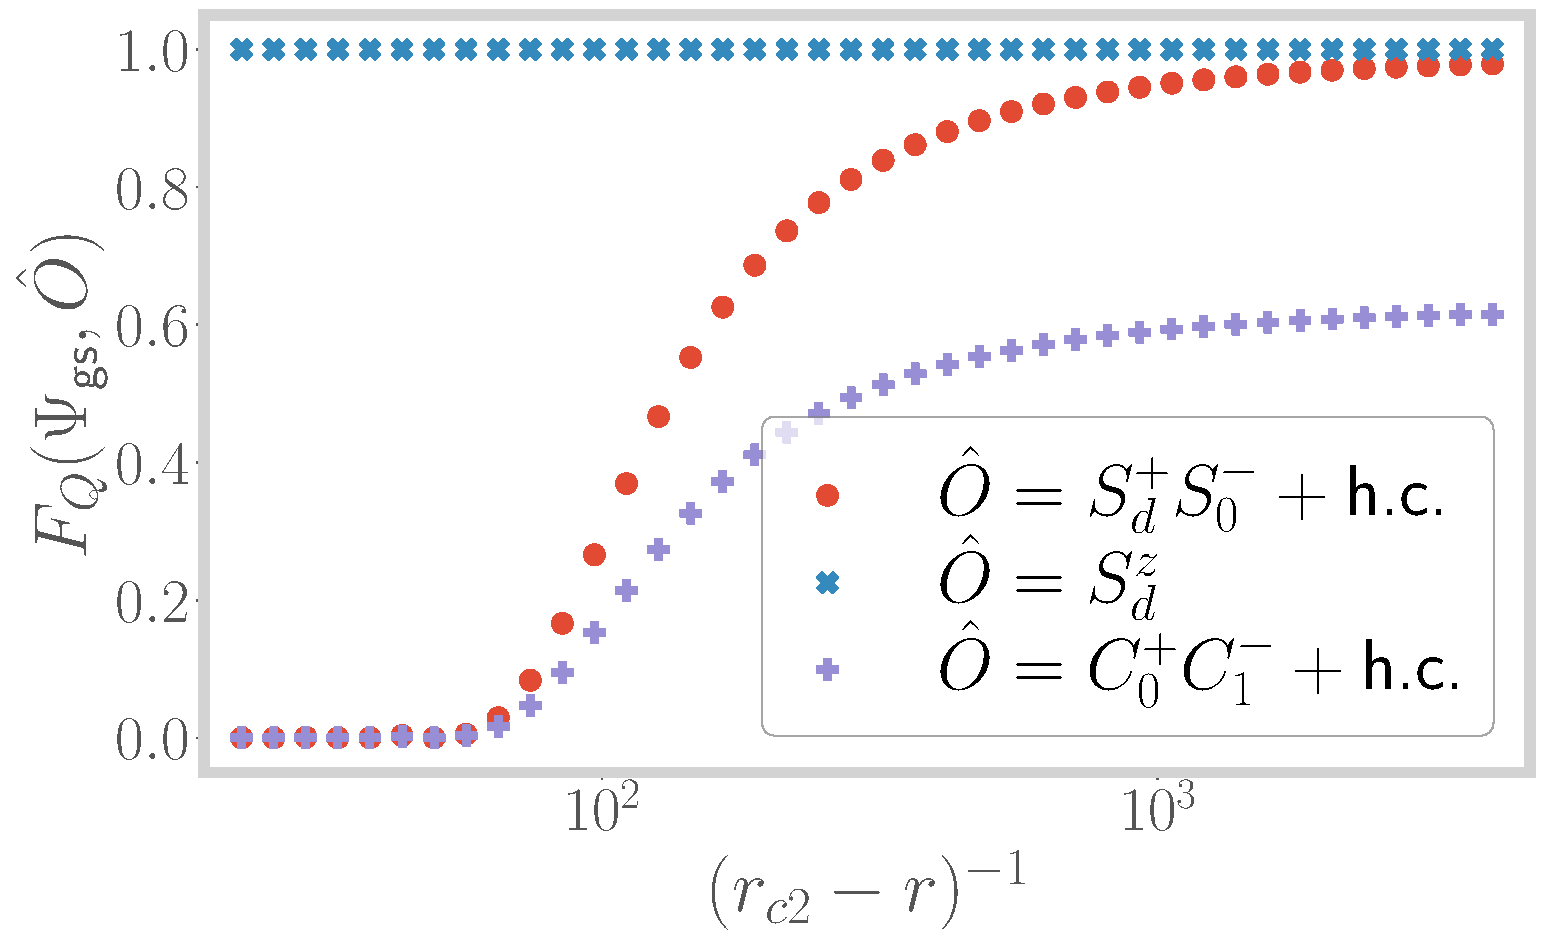
\includegraphics[width=0.48\textwidth]{rc2-QFI.pdf}
	\caption{{\it Left:} Variation of the quantum Fisher information for three separate fluctuations, across the entire range of \(r\). {\it Right:} The QFI corresponding to the same three operators, but very close to the QCP at \(r_{c2}\).}
	\label{QFI-esiam}
\end{figure}

For the sake of completeness, we generalise the above relations to finite temperatures by adopting the approach of Hauke et al.~\cite{Hauke2016}. For a mixed state at inverse temperature \(\beta\) characterised by the density matrix \(\rho = \sum_n f_n \ket{n}\bra{n}\) where \(\left(E_n,\ket{n}\right)\) are the eigenvalue-eigenstate pairs and \(f_n = e^{-\beta E_n}/\sum_n e^{-\beta E_n}\) are the Boltzmann weights, the FQI can be assigned a spectral representation of the form~\cite{Hauke2016}
\begin{eqnarray}
	F_Q(\rho, \hat O) = 2\sum_{m,n} \frac{\left(f_m - f_n\right)^2}{f_m + f_n}|\braket{m|\hat O|n}|^2~.
\end{eqnarray}
By using the identity \(\frac{f_m - f_n}{f_m + f_n} = \int_{-\infty}^\infty d\omega \delta(\omega + E_m - E_n)\tanh \left( \beta \omega/2 \right) \), the finite temperature FQI can be written in the form
\begin{eqnarray}\label{fqi-spectral}
	F_Q(\rho, \hat O) = 2\int_{-\infty}^\infty d\omega \tanh \left( \beta \omega/2 \right) \sum_{m,n} \left(f_m - f_n\right) \delta(\omega + E_m - E_n)|\braket{m|\hat O|n}|^2~.
\end{eqnarray}
In order to relate this with a correlation function, we now point out that the lesser Greens function \(G^<\) defined in eq.~\eqref{lesser-gf}, as well as the greater Greens function \(G^>\) that we will now define, also admit spectral representations in terms of the eigenstates \(\ket{n}\) of the full problem:
\begin{eqnarray}\label{lesser-spectral}
	G^<_{O^\dagger, O}(t) \equiv i\braket{\hat O^\dagger \hat O(t)} \implies & G^<_{O^\dagger, O}(\omega) = 2\pi i \sum_{m,n}f_n \delta(\omega + E_m - E_n) |\braket{m|\hat O^\dagger|n}|^2~,\\
	G^>_{O^\dagger, O}(t) \equiv -i\braket{\hat O(t) \hat O^\dagger} \implies & G^>_{O^\dagger, O}(\omega) = -2\pi i \sum_{m,n}f_m \delta(\omega + E_m - E_n) |\braket{m|\hat O|n}|^2~.
\end{eqnarray}
If \(\hat O\) is a Hermitian operator, eqs.~\eqref{lesser-spectral} can be used to rewrite the QFI in terms of \(G^\lessgtr_{O^\dagger, O}(\omega)\). Indeed, by combining eqs.~\eqref{lesser-spectral} and eq.~\eqref{fqi-spectral} with the assumption \(\hat O = \hat O^\dagger\), we get
\begin{eqnarray}
	F_Q(\rho, \hat O) = -\frac{1}{\pi i}\int_{-\infty}^\infty d\omega \tanh \left( \beta \omega/2 \right)\left(G^>_{O, O}(\omega) + G^<_{O, O}(\omega)\right)~. 
\end{eqnarray}
This constitutes the general relation between the finite temperature QFI for a general Hermitian many-particle operator \(\hat O\) and the corresponding many-particle correlations at zero and finite frequencies.

The Kubo linear response function associated with the operator \(\hat O(t)\) due to a perturbation from the same operator is associated with a correlation function/susceptibility \(\mathcal{C}_{\hat O}(t,t^\prime) = i\theta(t - t^\prime)\left< \left[\hat O(t), \hat O(t^\prime)\right] \right>\). By going to the frequency domain, the imaginary part of such a function can be related to the sum of the lesser and greater Greens functions:
\begin{eqnarray}
	\hspace*{2.2cm} \mathcal{C}_{\hat O}(\omega) &= i\int_0^\infty d(t-t^\prime) e^{i\omega(t-t^\prime)}\left( \left<\hat O(t) \hat O(t^\prime) \right> - \left<\hat O(t^\prime) \hat O(t) \right>\right)\nonumber \\
	\implies \mathcal{C}_{\hat O}(\omega) - \mathcal{C}_{\hat O}(\omega)^* &= i\int_0^\infty d(t-t^\prime)\left( e^{i\omega(t-t^\prime)}-e^{-i\omega(t-t^\prime)} \right)\left( \left<\hat O(t) \hat O(t^\prime) \right> - \left<\hat O(t^\prime) \hat O(t) \right>\right)\nonumber\\
						&= i\int_{-\infty}^{\infty}d(t-t^\prime) e^{i\omega(t-t^\prime)} \left( \left<\hat O(t) \hat O(t^\prime) \right> - \left<\hat O(t^\prime) \hat O(t) \right>\right)\nonumber \\
						&= -\left( G^>_{O,O}(\omega) + G^<_{O,O}(\omega) \right) 
\end{eqnarray}
This allows us to connect the QFI with the imaginary part of the Kubo correlation function/susceptibility obtained in Ref.\cite{Hauke2016}:
\begin{eqnarray}
F_Q(\rho, \hat O) = \frac{1}{\pi i}\int_{-\infty}^\infty d\omega \tanh \left( \beta \omega/2 \right)\left(\mathcal{C}_{\hat O}(\omega) - \mathcal{C}_{\hat O}(\omega)^*\right) ~.
\end{eqnarray}



\section{One-shot decoupling of impurity from zeroth site}
\label{app-imp-remove}
We will decouple the impurity states from the fixed point Hamiltonian using a single URG transformation. This will, of course, generate correlations on the zeroth site. The resulting Hamiltonian will be an AIM with the hopping between the zeroth site and the rest of the chain acting as the effective hybridisation. Schematically, we will have
\begin{eqnarray}
	H^* = H_\text{imp} + V_\text{imp-0} + H_\text{0} + H_\text{0-1} + H_\text{rest} ~ {\xrightarrow{\text{decouple imp.}}} & E_\text{imp} + \tilde H_\text{0} + H_\text{0-1} + H_\text{rest} \nonumber\\
															       &= H_\text{new imp} + V_\text{new imp - rest} + H_\text{rest}~.
\end{eqnarray}

Since the impurity is not coupled with any site beyond the zeroth site, the parts of the Hamiltonian that involve "rest" will not change in the process. This also means that the decoupling can be performed by looking at the smaller Hamiltonian
\begin{eqnarray}
	H_\text{imp+0} = H_\text{imp} + H_\text{0} + V_\text{imp-0} =& -\frac{U^*}{2}\left( \hat n_{d \uparrow} - \hat n_{d \downarrow} \right)^2 - U_b \left( \hat n_{0 \uparrow} - \hat n_{0 \downarrow} \right)^2 + J^*S_d^z S_0^z\nonumber\\
								    & + {V^*}\sum_\sigma \left(c^\dagger_{d\sigma}c_{0\sigma} + \text{h.c.}\right) + \frac{J^*}{2}\left( c^\dagger_{d \uparrow}c_{d \downarrow} c^\dagger_{0 \downarrow} c_{0 \uparrow} + \text{h.c.} \right)~.
\end{eqnarray}

\subsection{Renormalisation from \({V^*}\)}
From the off-diagonal term involving \({V^*}\), we generate the following term, in the particle sector for \(0\):
\begin{eqnarray}
\sum_\sigma c^\dagger_{0\sigma}c_{d\sigma} \frac{{V^*}^2}{\tilde \omega - H_d} c^\dagger_{d\sigma}c_{0\sigma} = \sum_\sigma c^\dagger_{0\sigma}c_{d\sigma} \frac{{V^*}^2}{\tilde \omega + \frac{U^*}{2}\left( 1 - \hat n_{d\bar\sigma} \right)^2 + U_b \hat n_{0\bar\sigma} + \frac{J^*}{4}\left( 1 - \hat n_{d\bar\sigma} \right) \hat n_{0\bar\sigma} } c^\dagger_{d\sigma}c_{0\sigma}~.
\end{eqnarray}
where \(\tilde \omega\) is the quantum fluctuation operator for the impurity site and \(H_d = -\frac{U^*}{2}\left( \hat n_{d \uparrow} - \hat n_{d \downarrow} \right)^2 - U_b \left( \hat n_{0 \uparrow} - \hat n_{0 \downarrow} \right)^2 + J^*S_d^z S_0^z \), is the diagonal part of the Hamiltonian for the imp+0 system. In order to resolve the operators in the denominator, we expand the unity in the numerator using the identity \(1 = \hat n_{d\bar\sigma}\hat n_{0\bar\sigma} + \hat n_{d\bar\sigma}\hat h_{0\bar\sigma} + \hat h_{d\bar\sigma}\hat n_{0\bar\sigma} + \hat h_{d\bar\sigma}\hat h_{0\bar\sigma}\), where \(\hat h = 1 - \hat n\) is hole operator. On Substituting this, we get
\begin{eqnarray}
	\sum_\sigma  c^\dagger_{0\sigma}c_{d\sigma} \frac{{V^*}^2}{\tilde \omega - H_d} c^\dagger_{d\sigma}c_{0\sigma} &= {V^*}^2 \sum_\sigma c^\dagger_{0\sigma}c_{d\sigma} \frac{\hat h_{d\bar\sigma}\hat h_{0\bar\sigma} + \hat h_{d\bar\sigma}\hat n_{0\bar\sigma} + \hat n_{d\bar\sigma}\hat h_{0\bar\sigma} + \hat n_{d\bar\sigma}\hat n_{0\bar\sigma}}{\tilde \omega + \frac{U^*}{2}\hat h_{d\bar\sigma} + U_b \hat n_{0\bar\sigma} + \frac{J^*}{4}\hat h_{d\bar\sigma} \hat n_{0\bar\sigma} } c^\dagger_{d\sigma}c_{0\sigma}\nonumber\\
														       &= {V^*}^2 \sum_\sigma \hat h_{d\sigma} \hat n_{0\sigma}\left[\frac{\hat h_{d\bar\sigma}\hat h_{0\bar\sigma}}{\tilde\omega_{00} + \frac{U^*}{2}} + \frac{\hat h_{d\bar\sigma}\hat n_{0\bar\sigma}}{\tilde\omega_{01} + \frac{U^*}{2} + U_b + \frac{J^*}{4}} + \frac{\hat n_{d\bar\sigma}\hat h_{0\bar\sigma}}{\tilde\omega_{10}} + \frac{\hat n_{d\bar\sigma}\hat n_{0\bar\sigma}}{\tilde\omega_{11} + U_b}\right]~.\qquad
\end{eqnarray}
\(\tilde\omega_{(0,1),(0,1)}\) represents the quantum fluctuation scale corresponding to the configuration in the numerator.

In order to "freeze" the impurity dynamics, we will substitute \(\hat n_{d\sigma} = \hat n_{d\bar\sigma} = \frac{1}{2}\), because of the \({Z}_2\) symmetry and the particle-hole symmetry of the impurity levels. This gives
\begin{eqnarray}
	\frac{1}{4}{V^*}^2 \sum_\sigma \hat n_{0\sigma} \left[\frac{\hat h_{0\bar\sigma}}{\tilde\omega_{00} + \frac{U^*}{2}} + \frac{\hat n_{0\bar\sigma}}{\tilde\omega_{01} + \frac{U^*}{2} + U_b + \frac{J^*}{4}} + \frac{\hat h_{0\bar\sigma}}{\tilde\omega_{10}} + \frac{\hat n_{0\bar\sigma}}{\tilde\omega_{11} + U_b}\right]~.
\end{eqnarray}

The state that most closely represents the metallic ground state is \(\bar \omega_{10}\), we take that as the reference quantum fluctuation scale \(\bar\omega\). It is of the order of \(\bar\omega \sim -\frac{J^*}{4} - \frac{U^*}{2} - U_b\). We will now relate the other scales to \(\bar\omega\) by expressing them in terms of the energy of the initial state:
\begin{eqnarray}
	\tilde\omega_{00} \sim -U_b = \bar\omega + \frac{J^*}{4} + \frac{U^*}{2}, ~\tilde\omega_{01} \sim 0 = \bar\omega + \frac{J^*}{4} + \frac{U^*}{2} + U_b, ~\tilde\omega_{11} \sim -\frac{U^*}{2} = \bar\omega + \frac{J^*}{4} + U_b~.
\end{eqnarray}
Substituting these gives
\begin{eqnarray}
	\frac{1}{4}{V^*}^2 \sum_\sigma \hat n_{0\sigma} \left[\hat h_{0\bar\sigma}\alpha_1 + \hat n_{0\bar\sigma}\alpha_2\right]~,
\end{eqnarray}
where \(\alpha_1 = \left(\bar\omega + U^* + \frac{J^*}{4}\right)^{-1} + \left(\bar\omega\right)^{-1}\) and \(\alpha_2 = \left(\bar\omega + U^* + 2U_b + \frac{J^*}{2}\right)^{-1} + \left(\bar\omega + 2U_b + \frac{J^*}{4}\right)^{-1}\).

Because of the particle-hole symmetry on the impurity as well as in the bath, the renormalisation from the hole sector is obtained simply by transforming \(\hat n \leftrightarrow \hat h\):
\begin{eqnarray}
	\frac{1}{4}{V^*}^2 \sum_\sigma \hat h_{0\sigma} \left[\hat n_{0\bar\sigma}\alpha_1 + \hat h_{0\bar\sigma}\alpha_2\right]~.
\end{eqnarray}
The total renormalisation arising from \(V\) is therefore 
\begin{eqnarray}
	\frac{1}{4}{V^*}^2 \sum_\sigma \left[\alpha_1 \left( \hat n_{0\sigma}\hat h_{0\bar\sigma} + \hat h_{0\sigma}\hat n_{0\bar\sigma}\right) + \alpha_2 \left( \hat n_{0\sigma}\hat n_{0\bar\sigma} + \hat h_{0\sigma}\hat h_{0\bar\sigma}\right)\right] = \frac{1}{2}{V^*}^2 \left(\alpha_1 - \alpha_2\right) \left(\hat n_{0 \uparrow} - \hat n_{0 \downarrow}\right)^2 + \text{constant}~.\qquad
\end{eqnarray}

\subsection{Renormalisation from \(J^*\)}
The renormalisation arising from decoupling the Kondo coupling has two terms. The first term arises when the spin of the zeroth site is initially up:
\begin{eqnarray}
	\frac{{J^*}^2}{4}c^\dagger_{d \downarrow}c_{d \uparrow} c^\dagger_{0 \uparrow}c_{0 \downarrow} \frac{1}{\tilde \omega - H_d} c^\dagger_{0 \downarrow}c_{0 \uparrow} c^\dagger_{d \uparrow}c_{d \downarrow} &= c^\dagger_{d \downarrow}c_{d \uparrow} c^\dagger_{0 \uparrow}c_{0 \downarrow} \frac{{J^*}^2/4}{\tilde \omega + \frac{U^*}{2} + U_b + \frac{J^*}{4}} c^\dagger_{0 \downarrow}c_{0 \uparrow} c^\dagger_{d \uparrow}c_{d \downarrow} \nonumber\\
																										   &= \frac{{J^*}^2}{4}\frac{\hat n_{d \downarrow} \hat h_{d \uparrow} \hat n_{ 0 \uparrow} \hat h_{0 \downarrow}}{\tilde \omega + \frac{U^*}{2} + U_b + \frac{J^*}{4}} ~.
\end{eqnarray}
The quantum fluctuation scale \(\tilde \omega\) for this process can be similarly related to \(\bar\omega\): \(\tilde\omega \sim -\frac{U^*}{2} - U_b - \frac{J^*}{4} = \bar\omega\). This gives
\begin{eqnarray}
	\frac{{J^*}^2}{4}\frac{\hat n_{d \downarrow} \hat h_{d \uparrow} \hat n_{ 0 \uparrow} \hat h_{0 \downarrow}}{\bar\omega + \frac{U^*}{2} + U_b + \frac{3J^*}{4}} = \frac{{J^*}^2}{16}\frac{\hat n_{ 0 \uparrow} \hat h_{0 \downarrow}}{\bar\omega + \frac{U^*}{2} + U_b + \frac{J^*}{4}}~,
\end{eqnarray}
as the renormalisation for this configuration. At the final step, we substituted \(\hat n_{d\sigma} = \hat h_{d\sigma} = \frac{1}{2}\). For the other configuration where the spin of the zeroth site is down, we get
\begin{eqnarray}
	\frac{{J^*}^2}{16}\frac{\hat n_{ 0 \downarrow} \hat h_{0 \uparrow}}{\bar\omega + \frac{U^*}{2} + U_b + \frac{J^*}{4}}~.
\end{eqnarray}
Adding both sectors, we get
\begin{eqnarray}
	\frac{{J^*}^2}{16}\frac{1}{\bar\omega + \frac{U^*}{2} + U_b + \frac{J^*}{4}} \left(\hat n_{ 0\uparrow} - \hat n_{0 \downarrow}\right)^2~.
\end{eqnarray}

\subsection{Total renormalisation}
Adding the contributions from both \(V^*\) and \(J^*\),  the net renormalisation is the generation of a local correlation term \(-U^\prime\left(\hat n_{ 0\uparrow} - \hat n_{0 \downarrow}\right)^2\) on the zeroth site, where \(U^\prime\) is given by
\begin{eqnarray}
	U^\prime = \frac{-{J^*}^2/16}{\bar\omega + \frac{U^*}{2} + U_b + \frac{J^*}{4}} - \frac{1}{2}{V^*}^2\left(\frac{1}{\bar\omega + U^* + \frac{J^*}{4}} + \frac{1}{\bar\omega} - \frac{1}{\bar\omega + U^* + 2U_b + \frac{J^*}{2}} - \frac{1}{\bar\omega + 2U_b + \frac{J^*}{4}}\right)~.
\end{eqnarray}
The effective Hamiltonian for the zeroth site is therefore
\begin{eqnarray}
	H_\text{0+rest} = \underbrace{-\left(U^\prime + U_b\right)\left(\hat n_{0\uparrow} - \hat n_{0\downarrow}\right)^2}_\text{new correlated impurity} \underbrace{- t\sum_{j\in \text{n.n. of 0},\atop{\sigma}}\left(c^\dagger_{0\sigma}c_{j\sigma} + \text{h.c.}\right)}_\text{hopping between new impurity \& new bath} \underbrace{-t \sum_{\left<i,j \right>}\left(c^\dagger_{i\sigma}c_{j\sigma} + \text{h.c.}\right)}_\text{K.E. of new bath}~.
\end{eqnarray}

\section{Effective Hamiltonian for the excitations within the Hubbard sidebands}

Beyond \(r_{c1}\), the Hubbard sidebands can be seen to separate from the central Kondo resonance in the impurity spectral function. These sidebands are broad, indicating that the impurity site is hybridising with the bath from within the sidebands, at high energies \(\omega \sim U/2\). These processes lead to the presence of gapless excitations within the rest of the bath, outside the Mott gap. To find the effective Hamiltonian for the rest of the bath (sites 1 and onwards), we will take the eigenstates of the two-site Hamiltonian \(H\)that reside within the sideband as our ground-states, and treat the hopping from the zeroth site to the rest of the bath as a perturbation. The two-site Hamiltonian is
\begin{eqnarray}
	H_\text{two site} = V\sum_\sigma\left(c^\dagger_{d\sigma} c_{0\sigma} + \text{h.c}\right) + J \vec{S}_d\cdot\vec{S}_0 - \frac{U}{2} \left( \hat n_{d \uparrow} - \hat n_{d\downarrow} \right)^2 + \frac{U}{2}~.
\end{eqnarray}
In order to align the doubly-occupied impurity level at the more conventional value of \(U/2\), we have shifted the Hamiltonian by the same constant value. The effect of \(U_b\) has been ignored because it is small compared to \(U\) at the frequencies pertinent to the physics of the sidebands. 
The two-site states that reside within the Hubbard sidebands are
\begin{eqnarray}\label{gs-sideband}
	\ket{\Psi_{cc}} \equiv \ket{c}_d\ket{c}_0; ~ ~ c \in \left\{0,2\right\}; ~ ~\ket{\Psi_\text{CS}} \equiv \frac{1}{\sqrt 2}\left(\ket{2}_d\ket{0}_0 - \ket{0}_d\ket{2}_0\right);\nonumber \\
	\ket{\Psi_{\sigma,c}} = \alpha\ket{\sigma}_d\ket{c}_0 + \sqrt{1 - \alpha^2}\ket{c}_d\ket{\sigma}_0; ~ \sigma \in \left\{\uparrow,\downarrow\right\}; \nonumber\\
	\ket{\Psi_\text{CT}} = \beta\frac{1}{\sqrt 2}\left(\ket{\uparrow}_d\ket{\downarrow}_0 - \ket{\downarrow}_d\ket{\uparrow}_0\right) + \sqrt{1 - \beta^2}\frac{1}{\sqrt 2}\left(\ket{2}_d\ket{0}_0 + \ket{0}_d\ket{2}_0\right),
\end{eqnarray}
where the coefficients of the eigenstates are given by
\begin{eqnarray}
	\alpha \simeq \frac{V}{\sqrt{V^2 + \left(E_\text{X1} + \frac{U}{2}\right)^2 }},  ~ \beta = \frac{2V}{\sqrt{4V^2 + \left(E_\text{CS} + \frac{U}{2} + \frac{3J}{4}\right)^2}}~.
\end{eqnarray}
The energies of the states are
\begin{eqnarray}
	E_\text{gs} \equiv E_{00} = E_{22} = E_{CS} = \frac{U}{2}, E_\text{X1} \equiv E_{\sigma,c} = \frac{U}{4} + \sqrt{V^2 + \frac{U^2}{16}}~, \nonumber\\
	E_\text{X2} \equiv E_\text{CS} = \frac{U}{4} - \frac{3J}{8} + \sqrt{4V^2 + \left(\frac{U}{4} + \frac{3J}{8}\right)^2}~.
\end{eqnarray}
The ground state (comprising the states shown in eq.~\eqref{gs-sideband}) is triply degenerate. In order to study the dynamics of the bath, we now introduce the perturbation \(H_I = -t\sum_\sigma \left( c^\dagger_{0\sigma}c_{1\sigma} + \text{h.c.}\right) \). We also take an expanded set of eigenstates \(\left\{\ket{\Psi_n}\otimes\ket{a}\right\}\), where \(\left\{\ket{\Psi_n}\right\}\) is the set of eigenstates of \(H_\text{two site}\), and \(\ket{a} \in \left\{ \ket{0}, \ket{\uparrow}, \ket{\downarrow}, \ket{2} \right\} \) represents the configuration of the first site. The eigenstates of \(H_\text{two site}\) are also eigenstates the total number operator \(\hat n_d + \hat n_0 + \hat n_1\), and since \(H_I\) does not conserve the total number, all odd order shifts are zero: \(\braket{\Psi_n | H_I^b | \Psi_n}, b=1,3,\ldots\), is zero for all the eigenstates. 

For the second order shift, we need to calculate the overlaps \(\braket{\Psi_m | H_I | \Psi_n}, m\neq n\) for \(n\) in the ground state. Since all three ground-states involve the impurity and zeroth sites in charge configuration (0 or 2), \(H_I\ket{\Psi}_n\) will result in states of the form \(\ket{0(2)}_d\ket{\sigma}_0\ket{a}_1\). This resulting state has non-zero overlap only with the part \(\sqrt{1 - \alpha^2}\ket{c}_d\ket{\sigma}_0\ket{a}\) of the expanded state \(\ket{\Psi_{\sigma,c}}\ket{a}\). The square of each such overlap is, therefore, \(t^2\left( 1 - \alpha^2 \right) \). 
\begin{itemize}
	\item Excitations from the ground-states \(\ket{\Psi_{00}}\ket{0}\) and \(\ket{\Psi_{22}}\ket{2}\) have zero overlap with any other state, such that the second order shifts in these states is zero.
	\item Excitations from the ground-states \(\ket{\Psi_{00}}\ket{\sigma}\) and \(\ket{\Psi_{22}}\ket{\sigma}\) have non zero overlap with one excited state each, such that the second order shift in these states are \(\gamma^2 \equiv t^2\left( 1 - \alpha^2 \right) / \left(E_\text{X1} - E_\text{gs}\right) \).
	\item Excitations from the remaining ground states have non-zero overlaps with two excited states each, such that the second order shift in these states are \(2\gamma^2\).
\end{itemize}
Upon dropping the zeroth order part (because it has no dynamics for the rest of the bath), the effective Hamiltonian at second order in \(t\) takes the form
\begin{eqnarray}
	H_\text{eff}^{(2)} = \gamma^2 &\left[\left(\ket{\Psi_{00}}\bra{\Psi_{00}} + \ket{\Psi_{22}}\bra{\Psi_{22}} + 2\ket{\Psi_\text{CS}}\bra{\Psi_\text{CS}}\right)\left(\sum_\sigma \ket{\sigma}_1\bra{\sigma}_1\right) \right.\nonumber \\
				      &\left.  + 2\left(\ket{\Psi_{22}}\bra{\Psi_{22}} + \ket{\Psi_\text{CS}}\bra{\Psi_\text{CS}}\right) \ket{0}_1\bra{0}_1+2\left(\ket{\Psi_{00}}\bra{\Psi_{00}} + \ket{\Psi_\text{CS}}\bra{\Psi_\text{CS}}\right)\ket{2}_1\bra{2}_1\right]~.
\end{eqnarray}
By using the completeness relation \(1 = \sum_\sigma \ket{\sigma}_1\bra{\sigma}_1 + \ket{0}_1\bra{0}_1 + \ket{2}_1\bra{2}_1\) of the Hilbert space of the first site, this evaluates to
\begin{eqnarray}
	H_\text{eff}^{(2)} = \text{constant} + \gamma^2 \left(\ket{\Psi_{22}}\bra{\Psi_{22}} - \ket{\Psi_{00}}\bra{\Psi_{00}} \right) \left(\ket{2}_1\bra{2}_1 - \ket{0}_1\bra{0}_1\right) ~,
\end{eqnarray}
where the "constant" term refers to operators that do not depend on the dynamics of the rest of the bath. By defining the charge isospin operator \(C^z\ket{2(0)} = +(-)\frac{1}{2}\ket{2(0)}\), the effective Hamiltonian can be written as (dropping the non-dynamical part)
\begin{eqnarray}
	H_\text{eff}^{(2)} = 4\gamma^2C_\text{tot}^z  C_1^z~,
\end{eqnarray}
where \(C_i^z\) is the charge isospin for site \(i\) and \(C_\text{tot}^z \equiv C_d^z + C_0^z\) is the z-component of the total charge isospin for the impurity and the zeroth sites.

The fourth order shift in the energy of the eigenstate \(\ket{\Psi_n}\) will be given by
\begin{eqnarray}
	E_{n}^{(4)} = \sum_{j,k,l} \frac{\left(H_I\right)_{nl}\left(H_I\right)_{lk}\left(H_I\right)_{kj}\left(H_I\right)_{jn}}{\left( E_l - E_n \right)\left( E_k - E_n \right)\left( E_j - E_n \right) } - E_n^{(2)} \left[\frac{\left(H_I\right)_{kn}}{E_k - E_n}\right]^2~,
\end{eqnarray}
where the matrix elements \(\left( H_I \right)_{in} \) are defined as \(\braket{i | H_I | n}\). This fourth-order shift vanishes for almost all the ground-states. For the remaining states, it becomes important to treat their degeneracy. The "appropriate" combinations of states that provide non-zero fourth order contribution are
\begin{eqnarray}
	\ket{+} = \sqrt{\frac{2}{3}}\ket{\Psi_{22}}\ket{0}_1 + \sqrt{\frac{1}{3}}\ket{\Psi_\text{CS}}\ket{2}_1, ~ ~\ket{-} = -\sqrt{\frac{2}{3}}\ket{\Psi_{00}}\ket{2}_1 + \sqrt{\frac{1}{3}}\ket{\Psi_\text{CS}}\ket{0}_1~.
\end{eqnarray}
Corresponding to these ground states, the fourth-order shift in the eigenvalue is
\begin{eqnarray}
	E^{(4)} = \frac{3\gamma^4 \alpha^2 \beta^2}{\left( 1 - \alpha^2 \right) \left( E_\text{X2} - E_\text{gs} \right) }~,
\end{eqnarray}
such that the fourth-order contribution to the effective Hamiltonian is
\begin{eqnarray}
	H_\text{eff}^{(4)} &= E^{(4)}\left(\ket{+}\bra{+} + \ket{-}\bra{-}\right) \nonumber\\
			   &= \frac{\gamma^4 \alpha^2 \beta^2}{\left( 1 - \alpha^2 \right) \left( E_\text{X2} - E_\text{gs} \right) } \left[- C_\text{tot}^z C_\text{tot}^2 C_1^z +\sqrt{2}\mathcal{P}_\text{tot}^{4}\left(C_0^+ - C_d^+\right)C_1^- + \text{h.c.}\right] ~.
\end{eqnarray}
The operator \(\mathcal{P}_\text{tot}^{4}\) acts on states belonging to the combined \(d+0\) Hilbert space and projects on to the \(\hat n_d + \hat n_0 = 4\) subspace.



\section{Behaviour of the Kondo scale $T_K$ close to the transition}
\label{app-Tk}
Towards obtaining the emergent Kondo temperature scale $T_K$ close to the transition, we follow the approach used by Moeller et al. 1995~\cite{moeller_1995} and Held et al. 2013~\cite{held_2013}. Near the transition, they obtained a Kondo model from the full AIM by applying a Schrieffer-Wolff transition that removes the charge fluctuations of the impurity site and retains the physics of only the s-d coupling \(J\). This amounts to removing the side peaks from the impurity spectral function and focusing on the low-energy central peak. Held et al. then integrated the RG equation for this Kondo model by using a Lorentzian DOS in the bath. This is motivated by the fact that the central peak of the impurity spectral function is a Lorentzian, and the bath becomes equivalent to the impurity site under self-consistency. We implement the same approach but on our extended impurity model, such that the transformation then leads to a \(J-U_b\) model. The relevant RG equations are mentioned in Section IV of the main manuscript:
\begin{eqnarray}
	\Delta J = -\frac{n_j J\left(J + 4U_b\right)}{\omega - D/2 + U_b/2 + J/4},~~ \Delta U_b = 0~,
\end{eqnarray}
where \(n_j = \rho(D)|\Delta D|\) is proportional to the bath density of states. In Section VII of the main manuscript, we show that the spectral function of the zeroth site is tracked by that on the impurity site through the coherent spin-flip fluctuations, and this shows that the appropriate density of states for the bath in this regime is of the Lorentzian kind (same as the shape of the central peak of the impurity spectral function). We therefore set
\begin{eqnarray}
	\rho(D) = \frac{\rho_0 \Gamma^2}{D^2 + \Gamma^2}~,
\end{eqnarray}
where \(\Gamma\) represents the half-width of the Lorentzian. A similar line of arguments was presented by Held et al.~\cite{held_2013}. Close to the transition, the RG flow of the Kondo coupling \(J\) is stunted by the competing pairing term, and the RG equation can be simplified into the Poor man's scaling \(1-\)loop form:
\begin{eqnarray}
	\frac{d J}{d D} \simeq -2\rho_0 \Gamma^2\frac{J\left(J + 4U_b\right)}{\left( \Gamma^2 + D^2 \right) D}~.
\end{eqnarray}
We now integrate this RG equation over the range \(D \in \left[D_0, D^*\right] \), where \(D_0\) is the bare bandwidth, and \(D^*\) is the fixed-point bandwidth. \(D^*\) represents the energy scale for the conduction electrons in the IR.
\begin{eqnarray}
	\int_{J_0}^{J^*} \frac{d J}{J\left(J + 4U_b\right)} = -\int_{D_0}^{D^*}\frac{2\rho_0 \Gamma^2 d D}{\left( \Gamma^2 + D^2 \right) D} \nonumber\\
	\implies \frac{1}{4 U_b \rho_0} \left(\ln \frac{J^*}{J_0} - \ln \frac{J^* + 4U_b}{J_0 + 4 U_b}\right) = \ln \frac{D^* + \Gamma^2}{D_0 + \Gamma^2} - \ln \frac{D^*}{D_0}~.
\end{eqnarray}
We will now take the limit of \(J_0 + 4U_b \to 0^-\) and {\it equate the singular terms on both sides} of the equation:
\begin{eqnarray}
	\ln \frac{D^*}{D_0} = -\frac{1}{4 U_b \rho_0} \ln \frac{J_0 + 4 U_b}{J_0} = -\frac{1}{4 U_b \rho_0} \ln \left(r_{c2} - r\right) + \text{non-singular part}~.
\end{eqnarray}
We have replaced the couplings \(J\) and \(U_b\) with the dimensionless parameters \(r = -U_b/J_0\) and \(r_{c2} = 1/4\). Dropping the non-singular part and solving for \(D^*\) then gives the IR energy scale:
\begin{eqnarray}
	D^* = D_0 \exp\left[-\frac{\ln\left( r_{c2} - r \right)}{4 U_b \rho_0}\right]~.
\end{eqnarray}
The dynamically generated Kondo temperature scale is then obtained as
\begin{eqnarray}
	T_K = \frac{D^*}{k_B} = \frac{D_0}{k_B} \exp\left[-\frac{\ln\left( r_{c2} - r \right)}{4 U_b \rho_0}\right]~.
\end{eqnarray}
Note that the prefactor of the logarithm is positive because \(U_b\) is negative: \(-4U_b\rho_0 = |4U_b \rho_0|\). As we approach the transition, the parameter \(r\) takes the limit \(r \to r_{c2}^-\), and the Kondo temperature scale vanishes:
\begin{eqnarray}
	\lim_{r \to r_{c2}^-} T_K = \frac{D_0}{k_B} \lim_{r \to r_{c2}^-}\left(r_{c2} - r\right)^{4|U_b\rho_0|} \to 0~.
\end{eqnarray}


\section{Effective Hamiltonian for the low-lying excitations at the critical point}
\label{app-nfl}

In order to obtain an effective Hamiltonian for the low-lying excitations in the bath, we will introduce a hopping term \(V\) between the zeroth site and the first site into the two-site Hamiltonian \(H_0\), and treat that term perturbatively. 
\begin{eqnarray}
	H = \underbrace{J \vec{S}_d\cdot\vec{S}_0 - U_b \left( \hat n_{0 \uparrow} - \hat n_{0 \downarrow} \right)^2 }_{H_0} \underbrace{- t\sum_\sigma\left( c^\dagger_{0\sigma}c_{1\sigma} + \text{h.c.}\right)}_V~.
\end{eqnarray}
As mentioned before, \(H_0\) is our zeroth Hamiltonian, while \(V\) is the perturbation. At the critical point, the zeroth Hamiltonian has a \(20-\)fold degenerate ground-state manifold, and we will show later that it is this degeneracy that leads to NFL excitations. The ground-states are
\begin{eqnarray}
	\left\{\ket{S=S^z=0}, \ket{\uparrow, 0}, \ket{\uparrow, 2}, \ket{\downarrow, 0}, \ket{\downarrow, 2}\right\}\otimes\left\{\ket{0},\ket{\uparrow},\ket{\downarrow},\ket{\uparrow \downarrow}\right\}~.
\end{eqnarray}
The ket to the left of \(\otimes\) describes the configuration of the impurity and zeroth sites; \(S=S^z=0\) represents the singlet, while the remaining four states \(\ket{\sigma, 0},\ket{\sigma,2}\) are local moment states. The ket to the right of \(\otimes\) represents the configuration of the first site. Eight of these states have zero matrix elements within the ground-state subspace, even in the presence of the perturbation, so we drop these states. Since the full Hamiltonian conserves the total number of particles \(N_\text{tot} = \sum_\sigma\left(\hat n_{d\sigma} + \hat n_{0\sigma} + \hat n_{1\sigma}\right)\) and the total spin \(S_\text{tot}^z = S_d^z + S_0^z + S_1^z\), the remaining 12 states can be split into decoupled blocks based on the values of these two operators:
\begin{eqnarray}
	N_\text{tot} = c+2, S_\text{tot}^z = 0&: \ket{S=S^z=0}\ket{c}, \ket{\uparrow, c, \downarrow}, \ket{\downarrow, c, \uparrow}; ~c=0,2, \nonumber\\
	N_\text{tot} = 3, S_\text{tot}^z = \pm\frac{1}{2}&: \ket{S=S^z=0}\ket{\sigma}, \ket{\sigma, 0, 2}, \ket{\sigma, 2, 0};\sigma=\uparrow,\downarrow~.
\end{eqnarray}
The perturbation \(V\) will lift the degeneracy in each block; to calculate the modified spectrum, we diagonalise each block in the presence of \(V\). We will first write down the action of the perturbation on the singlet ground-states: this will make it easier to identify the true eigenstates.
\begin{eqnarray}
	N_\text{tot} = c+2, S_\text{tot}^z = 0 &: V\ket{\text{SS}_c} = \frac{t}{\sqrt 2}\left( \ket{\downarrow,c,\uparrow} - \ket{\uparrow,c,\downarrow} \right),~ c=0,2,\nonumber\\
	N_\text{tot} = 3, S_\text{tot}^z = \frac{\sigma}{2} &: V\ket{\text{SS}_\sigma} = \frac{t}{\sqrt 2}\ket{\sigma}\otimes\left(\ket{0,2} + \ket{2,0}\right),~\sigma=\uparrow(1),\downarrow(-1)~,
\end{eqnarray}
where we have introduced the notation \(\ket{\text{SS}_{\alpha}} = \ket{S=S^z=0}\otimes\ket{\alpha},\alpha=0,\uparrow,\downarrow,2\). This shows that the action of the perturbation on the singlet state is to create linear combinations of the local moment states in the respective blocks. We therefore define the two possible linear combinations \(\ket{\text{LM}_\pm^{N_\text{tot},S_\text{tot}^z}}\) within each block:
\begin{eqnarray}
	N_\text{tot} = c+2, S_\text{tot}^z = 0 &: \ket{\text{LM}_\pm^{c+2,0}} = \frac{1}{\sqrt 2}\left(\ket{\uparrow, c, \downarrow} \pm \ket{\downarrow, c, \uparrow}\right),~c=0,2,\nonumber\\
	N_\text{tot} = 3, S_\text{tot}^z = \frac{\sigma}{2} &: \ket{\text{LM}_{\sigma}^{3,\frac{1}{2}}} = \frac{1}{\sqrt 2}\left(\ket{\sigma, 0, 2} \pm \ket{\sigma, 2, 0}\right),~\sigma=\uparrow(1), \downarrow(-1)~.
\end{eqnarray}
In terms of these linear combinations, we then get
\begin{eqnarray}
	V\ket{\text{SS}_0} = t\ket{\text{LM}_-^{2,0}}, ~ ~ V\ket{\text{LM}_-^{2,0}} = t\ket{\text{SS}_0}, ~ ~V\ket{\text{LM}_+^{2,0}} = 0; \quad V\ket{\text{SS}_\uparrow} = t\ket{\text{LM}_+^{3, \uparrow}},\nonumber \\
	V\ket{\text{LM}_+^{3, \uparrow}} = t\ket{\text{SS}_\uparrow}, ~ ~V\ket{\text{LM}_-^{3, \uparrow}} = 0, ~ ~ V\ket{\text{SS}_\downarrow} = t\ket{\text{LM}_+^{3, \downarrow}}, ~ ~ V\ket{\text{LM}_+^{3, \downarrow}} = t\ket{\text{SS}_\downarrow},\nonumber \\
	V\ket{\text{LM}_-^{3, \downarrow}} = 0; \quad V\ket{\text{SS}_2} = t\ket{\text{LM}_-^{4,0}}, ~ ~ V\ket{\text{LM}_-^{4,0}} = t\ket{\text{SS}_2}, ~ ~V\ket{\text{LM}_+^{4,0}} = 0~.
\end{eqnarray}
The zero matrix elements at the far right of each line should be understood as the fact that \(V\) takes those states out of the ground-state subspace. For e.g., the state \(V\ket{\text{LM}_-^{2,0}}\) is not really zero, but the overlap of \(V\ket{\text{LM}_-^{2,0}}\) with any other state in the ground-state subspace spanned by the 20 degenerate states is zero. We now see that each of the \(3\times3\) blocks decouples into a \(2\times2\) block \(\begin{pmatrix} 0 & t \\ t & 0 \end{pmatrix} \)and a \(1\times1\) block \(\begin{pmatrix} 0 \end{pmatrix} \) when written in terms of the linear combinations \(\ket{\text{LM}_\pm}\). The state in the final block is therefore already an eigenstate, but with zero energy, so that will drop out from the effective Hamiltonian. The remaining \(2\times 2\) block has eigenstates \(\ket{\pm^{N_\text{tot},S_\text{tot}^z}}\) that are linear combinations of the singlet states and the surviving local moment combination, with eigenvalues \(\pm t\):
\begin{eqnarray}
	\label{new g-states}
	N_\text{tot} = 2, S_\text{tot}^z = 0: \ket{\pm^{2,0}} = \frac{1}{\sqrt 2}\left(\ket{\text{SS}_0} \pm \ket{\text{LM}_-^{2,0}}\right),\nonumber \\
	N_\text{tot} = 3, S_\text{tot}^z = \frac{1}{2}: \ket{\pm^{3,\frac{1}{2}}} = \frac{1}{\sqrt 2}\left(\ket{\text{SS}_\uparrow} \pm \ket{\text{LM}_+^{3,\frac{1}{2}}}\right),\nonumber \\
	N_\text{tot} = 3, S_\text{tot}^z = -\frac{1}{2}: \ket{\pm^{3,-\frac{1}{2}}} = \frac{1}{\sqrt 2}\left(\ket{\text{SS}_\downarrow} \pm \ket{\text{LM}_+^{3,-\frac{1}{2}}}\right), \nonumber\\
	N_\text{tot} = 4, S_\text{tot}^z = 0: \ket{\pm^{4,0}} = \frac{1}{\sqrt 2}\left(\ket{\text{SS}_2} \pm \ket{\text{LM}_-^{4,0}}\right)~.
\end{eqnarray}
At this point, it is worth noting that the polarised ground-states \(\ket{S_\text{tot}^z=\sigma\frac{1}{2}},\sigma=\pm 1\) can be written as an equal superposition of the singlet states \(\ket{\text{SS}}_{d0}\otimes\ket{\sigma}_1\) and the local moment states \(\frac{1}{\sqrt 2}\left(\ket{\sigma, 0, 2} - \ket{\sigma, 2, 0}\right)\). The polarised symmetry-broken states therefore act as a bridge between the ground states of the two phases and are important in displaying the breakdown of the Kondo cloud at the QCP and the consequences arising from it (like inexact screening of the impurity and fractional magnetisation and entanglement entropy, which will be discussed in the next section).

By combining the two eigenstates \(\ket{\pm}\) for each block, one can then reconstruct the effective Hamiltonian \(\mathcal{H}^{N_\text{tot}, S_\text{tot}^z}_\text{eff}\) that describes the dynamics of the first site from within the ground-state subspace of the zeroth Hamiltonian. Formally, this is written as
\begin{eqnarray}
	\label{eff-ham-all}
	\mathcal{H}^{N_\text{tot}, S_\text{tot}^z}_\text{eff} &=& t\ket{+^{N_\text{tot}, S_\text{tot}^z}}\bra{+^{N_\text{tot}, S_\text{tot}^z}} - t\ket{-^{N_\text{tot}, S_\text{tot}^z}}\bra{-^{N_\text{tot}, S_\text{tot}^z}}~, \nonumber\\
							      &=& \begin{cases} t \left[\ket{\text{SS}_\alpha}\bra{\text{LM}_-^{N_\text{tot}, S_\text{tot}^z}} + \ket{\text{LM}_-^{N_\text{tot}, S_\text{tot}^z}}\bra{\text{SS}_\alpha}\right], ~ ~ \alpha=0,2~,\\
	t \left[\ket{\text{SS}_\alpha}\bra{\text{LM}_+^{N_\text{tot}, S_\text{tot}^z}} + \ket{\text{LM}_+^{N_\text{tot}, S_\text{tot}^z}}\bra{\text{SS}_\alpha}\right], ~ ~ \alpha=\uparrow, \downarrow~.\\
        \end{cases}
\end{eqnarray}
We first write down the effective Hamiltonian for \(\alpha=0\) which corresponds to \(N_\text{tot}=2, S_\text{tot}^z = 0\):
\begin{eqnarray}
	\mathcal{H}^{2, 0}_\text{eff} = t \left[\ket{\text{SS}_0}\bra{\text{LM}_-^{2,0}} + \ket{\text{LM}_-^{2,0}}\bra{\text{SS}_0}\right] ~.
\end{eqnarray}
In order to convert this into a second-quantised form, we will use the following identities:
\begin{eqnarray}
	\ket{\text{SS}_0} &= \frac{1}{\sqrt 2}\left(P_d^{ \uparrow} c^\dagger_{0 \downarrow} - P_d^{ \downarrow} c^\dagger_{0 \uparrow} \right) P_0^{(0)}P_1^{(0)}\ket{0}; \quad \ket{\text{LM}_-^{2,0}} &= \frac{1}{\sqrt 2}\left(P_d^{ \uparrow} c^\dagger_{1 \downarrow} - P_d^{ \downarrow} c^\dagger_{1 \uparrow} \right) P_0^{(0)}P_1^{(0)}\ket{0}~,
\end{eqnarray}
where \(P_i^{(m)} (m=0,1,2)\) projects onto the \(\hat n_i = m\) subspace on the i\(^\text{th}\) site, and \(P_d^\sigma\) projects the impurity spin into \(\ket{\sigma};\sigma=\uparrow,\downarrow\) configuration.
We then have
\begin{eqnarray}
	\ket{\text{SS}_0} \bra{\text{LM}_-^{2,0}} &= \frac{1}{2}\left(P_d^{\uparrow} c^\dagger_{0 \downarrow} - P_{d}^{\downarrow} c^\dagger_{0 \uparrow} \right)P_0^{(0)}P_1^{(0)}\left(P_{d}^{\uparrow} c_{1 \downarrow} - P_{d}^{\downarrow} c_{1 \uparrow} \right)\nonumber \\
						  &= P_1^{(0)}\frac{1}{2}\left(P_d^\uparrow c^\dagger_{0 \downarrow}c_{1 \downarrow} + P_d^\downarrow c^\dagger_{0 \uparrow}c_{1 \uparrow} - S_d^+ c^\dagger_{0 \downarrow} c_{1 \uparrow} - S_d^- c^\dagger_{ 0 \uparrow} c_{1 \downarrow}\right)P_0^{(0)}~,
\end{eqnarray}
where we have used \(P^2 = P\) if \(P\) is a projector, and that \(P_d^\uparrow P_d^ \downarrow = S_d^+\). Substituting these into the effective Hamiltonian and recognising that \(P_d^\uparrow = \frac{1}{2} + S_d^z, P_d^\downarrow = \frac{1}{2} - S_d^z\) gives
\begin{eqnarray}
	\mathcal{H}^{2, 0}_\text{eff} = \frac{t}{2}&\left[\left(\frac{1}{2} + S_d^z\right) c^\dagger_{0 \downarrow} P_0^{(0)} P_1^{(0)} c_{1 \downarrow} -S_d^+ c^\dagger_{0 \downarrow} P_0^{(0)} P_1^{(0)} c_{1 \uparrow} - S_d^- c^\dagger_{0 \uparrow} P_0^{(0)} P_1^{(0)} c_{1 \downarrow} \right. \nonumber\\
						   &\left.+ \left(\frac{1}{2} - S_d^z\right) c^\dagger_{0 \uparrow} P_0^{(0)} P_1^{(0)} c_{1 \uparrow} \right] + \text{h.c.}~.
\end{eqnarray}
In order to make this more illuminating, we define the holon excitation operators \(h^\dagger_{i\sigma} = c^\dagger_{i\sigma}P_i^{(0)}\). In terms of these operators, the effective Hamiltonian becomes
\begin{eqnarray}
	\mathcal{H}^{2, 0}_\text{eff} &=& \frac{t}{2}\left[\left(\frac{1}{2} + S_d^z\right) \left(h^\dagger_{0 \downarrow} h_{1 \downarrow} + h^\dagger_{1 \downarrow} h_{0 \downarrow}\right) - S_d^+ \left(h^\dagger_{0 \downarrow} h_{1 \uparrow} + h^\dagger_{1 \downarrow} h_{0 \uparrow}\right) - S_d^- \left(h^\dagger_{0 \uparrow} h_{1 \downarrow} + h^\dagger_{1 \uparrow} h_{0 \downarrow}\right) + \right. \nonumber\\
				      & & \left. \left(\frac{1}{2} - S_d^z\right) \left(h^\dagger_{0 \uparrow} h_{1 \uparrow}+ h^\dagger_{1 \uparrow} h_{0 \uparrow}\right) \right]\nonumber\\
				      &=& -t\left[S_d^z\frac{1}{2}\left(h^\dagger_{0 \uparrow} h_{1 \uparrow}+ h^\dagger_{1 \uparrow} h_{0 \uparrow} - h^\dagger_{0 \downarrow} h_{1 \downarrow} - h^\dagger_{1 \downarrow} h_{0 \downarrow}\right) + \frac{1}{2}S_d^+ \left(h^\dagger_{0 \downarrow} h_{1 \uparrow} + h^\dagger_{1 \downarrow} h_{0 \uparrow}\right) \right. \nonumber\\
				      &+& \left.\frac{1}{2}S_d^- \left(h^\dagger_{0 \uparrow} h_{1 \downarrow} + h^\dagger_{1 \uparrow} h_{0 \downarrow}\right) \right] + \frac{t}{4}\left(h^\dagger_{0 \uparrow} h_{1 \uparrow}+ h^\dagger_{1 \uparrow} h_{0 \uparrow} + h^\dagger_{0 \downarrow} h_{1 \downarrow} + h^\dagger_{1 \downarrow} h_{0 \downarrow}\right) \label{eff-ham-nfl}~.
\end{eqnarray}
The first part of the Hamiltonian (with a \(-t\) factor in front) is reminiscent of a two-spin Heisenberg Hamiltonian. To investigate this, we write down the potential second spin:
\begin{eqnarray}
	\mathcal{S}^z_1 \equiv \frac{1}{2}\left(h^\dagger_{0 \uparrow} h_{1 \uparrow}+ h^\dagger_{1 \uparrow} h_{0 \uparrow} - h^\dagger_{0 \downarrow} h_{1 \downarrow} - h^\dagger_{1 \downarrow} h_{0 \downarrow}\right)~.
\end{eqnarray}
Note that each term that comprises the full operator \(\mathcal{S}^z_1\) has a combined projector \(P_{01}^{(0)} = P_0^{(0)}P_1^{(0)} = P_1^{(0)}P_0^{(0)}\) in the middle with a single annihilation operator to the right. This means that \(\mathcal{S}^z\) projects onto the smaller set of only those states that satisfy \(\hat n_0 + \hat n_1 = 1\). That is also the meaning of the subscript \(1\) in \(\mathcal{S}^z_1\). There are four such states: \(\ket{\uparrow, 0}, \ket{\downarrow,0}, \ket{0,\uparrow}, \ket{0, \downarrow}\). In fact, it is easy to see that the eigenstates of \(\mathcal{S}^z\) are
\begin{eqnarray}
	\label{sigmaz-def}
	\ket{\Uparrow}_{1,\pm} &= \frac{1}{\sqrt 2}\left(\ket{\uparrow,0} \pm \ket{0, \uparrow}\right), \quad \mathcal{S}^z_1\ket{\Uparrow}_{1,\pm} = \pm\frac{1}{2}\ket{\Uparrow}_{1,\pm}, \\
	\ket{\Downarrow}_{1,\pm} &= \frac{1}{\sqrt 2}\left( \ket{\downarrow, 0} \pm \ket{0, \downarrow}\right),\quad \mathcal{S}^z_1\ket{\Downarrow}_{1,\pm} = \mp\frac{1}{2}\ket{\Downarrow}_{1,\pm}~.
\end{eqnarray}
The label \(\pm\) on top of the eigenstates indicates that these are also eigenstates of the parity operator \(\mathcal{P}_{01}\) that switches the site labels \(0\) and \(1\):
\begin{eqnarray}
	\label{parity-define}
	\mathcal{P}_{01}\ket{\alpha,\alpha^\prime} = \ket{\alpha^\prime,\alpha};~~ \alpha,\alpha^\prime \in \left\{0,\uparrow,\downarrow,2\right\} ~.
\end{eqnarray}
In fact, the eigenstates \(\ket{\Uparrow}_{1,+1}\) and \(\ket{\Downarrow}_{1,-1}\) both have \(\mathcal{S}^z = \frac{1}{2}\), but are orthogonal because they have different parities. Analogous to the \(\mathcal{S}_1^z\) operator, we can also read off the potential \(\mathcal{S}_1^\pm\) ladder operators from the effective Hamiltonian:
\begin{eqnarray}
	\label{sigmapm-def}
	\mathcal{S}_1^+ = h^\dagger_{0 \uparrow} h_{1 \downarrow} + h^\dagger_{1 \uparrow} h_{0 \downarrow}, ~ ~ ~\mathcal{S}_1^- = \left(\mathcal{S}_1^+\right)^\dagger~.
\end{eqnarray}
Applying these ladder operators on the eigenstates of \(\mathcal{S}_1^z\) gives
\begin{eqnarray}
	\mathcal{S}_1^+ \ket{\Downarrow}_{1,\pm} = \pm \ket{\Uparrow}_{1,\pm}; \quad\mathcal{S}_1^- \ket{\Uparrow}_{1,\pm} = \pm \ket{\Downarrow}_{1,\pm}; \quad\mathcal{S}_1^+ \ket{\Uparrow}_{1,\pm} = \mathcal{S}_1^- \ket{\Downarrow}_{1,\pm} = 0~.
\end{eqnarray}
This makes it clear that the pair of states \(\ket{\Uparrow}^{+}_1\) and \(\ket{\Downarrow}^{+}_1\) form a spin-half doublet, as does the other pair \(\ket{\Uparrow}^{-}_1\) and \(\ket{\Downarrow}^{-}_1\). We can define new spin operators that act only on a single parity subspace:
\begin{eqnarray}
	\mathcal{S}^a_{1,\pm} = \pm \mathcal{S}^a ~\frac{1}{2}\left(1 \pm \mathcal{P}_{01}\right);~ ~ a=x,y,z~.
\end{eqnarray}
The operator \(\frac{1}{2}\left(1 \pm \mathcal{P}_{01}\right)\) projects on to the subspace with \(\pm 1\) parity. In the notation \(\mathcal{S}^a_{1,\pm}\), the label \(\pm\) indicates the parity sector to which the operator applies, while 1 indicates that we are operating in the subspace with \(\hat n_0 + \hat n_1 = 1\). Two operators corresponding to different parity subspaces will commute because they act on disjoint Hilbert spaces: \(\left[\mathcal{S}^a_{+1}, \mathcal{S}^b_{-1}\right] = 0\). In terms of these projected spin operators, we recover the usual spin-half SU(2) algebra:
\begin{eqnarray}
	\mathcal{S}^z_{1,\pm} \ket{\Uparrow}_{1,\pm} = \frac{1}{2}\ket{\Uparrow}_{1,\pm}; \quad\mathcal{S}^z_{1,\pm}\ket{\Downarrow}_{1,\pm} = -\frac{1}{2}\ket{\Downarrow}_{1,\pm};\nonumber\\
	\mathcal{S}^+_{1,\pm} \ket{\Downarrow}_{1,\pm} = \ket{\Uparrow}_{1,\pm}; \quad\mathcal{S}^-_{1,\pm} \ket{\Uparrow}_{1,\pm} = \ket{\Downarrow}_{1,\pm}.\qquad
\end{eqnarray}
The part of the effective Hamiltonian that involves the impurity can now be written in terms of these new spin operators:
\begin{eqnarray}
	t\left(\vec{S}_d\cdot\vec{\mathcal{S}}_{-,1} - \vec{S}_d\cdot\vec{\mathcal{S}}_{+,1}\right); ~ ~ \vec{\mathcal{S}}_{\pm} = \left(\mathcal{S}_{\pm}^x ~ ~ \mathcal{S}_{\pm}^y ~ ~\mathcal{S}_{\pm}^z\right)~.
\end{eqnarray}
The last term in eq.~\eqref{eff-ham-nfl} (with a prefactor of \(\frac{t}{4}\)) can now be identified as the parity operator \(\mathcal{P}_{01}\) acting within the subspace \(\hat n_0 + \hat n_1 = 1\), because it has eigenstates \(\ket{\uparrow,0}\pm\ket{0,\uparrow}\) and \(\ket{\downarrow,0}\pm\ket{0,\downarrow}\) with eigenvalues \(\pm 1\). The full effective Hamiltonian in the \(N_\text{tot}=2\) subspace then takes the compact form
\begin{eqnarray}
	\mathcal{H}^{2, 0}_\text{eff} = t\left(\vec{S}_d\cdot\vec{\mathcal{S}}_{1,-1} - \vec{S}_d\cdot\vec{\mathcal{S}}_{1,+}\right) + \frac{t}{4}\mathcal{P}_{01} P_{01}^{(1)}~,
\end{eqnarray}
where \(P_{01}^{(1)} = P_{0}^{(1)}P_{1}^{(0)} + P_{0}^{(0)}P_{1}^{(1)}\) projects on to the \(\hat n_0 + \hat n_1 = 1\) subspace. In light of these new spin operators, the original eigenstates \(\ket{\pm^{2,0}}\) can be written in terms of these emergent spins \(\ket{\Uparrow}_{1,\pm}\) and \(\ket{\Downarrow}_{1,\pm}\):
\begin{eqnarray}
	\ket{\pm^{2,0}} &=& \frac{1}{2}\left(\ket{\uparrow,\downarrow,0} - \ket{\downarrow,\uparrow,0} \pm \ket{\uparrow,0,\downarrow} \mp \ket{\downarrow,0,\uparrow}\right) = \frac{1}{2}\left[\ket{\uparrow}\left(\ket{\downarrow,0} \pm \ket{0, \downarrow}\right) - \ket{\downarrow}\left(\ket{\uparrow,0} \pm \ket{0,\uparrow}\right)\right] \nonumber\\
			    &=& \frac{1}{\sqrt 2}\left( \ket{\uparrow}\ket{\Downarrow}_{1,\pm} - \ket{\downarrow}\ket{\Uparrow}_{1,\pm} \right)~.
\end{eqnarray}
Both the ground and excited states are therefore spin-singlet states, but they belong to the negative and positive parity sectors respectively.

We now proceed to the \(N_\text{tot}=4\) sector, which is equivalent to \(\alpha=2\) and \(\hat n_0 + \hat n_1 = 3\). From eq.~\eqref{eff-ham-all}, we note that the effective Hamiltonian of the \(\alpha=2\) sector is obtained from that of the \(\alpha=0\) sector by replacing the holons with doublons, \(\ket{0} \to \ket{2}\). This allows us to use the results of the \(N_\text{tot}=2\) sector simply by making the above-mentioned holon-doublon transformation. Accordingly, the composite up and down spins of the \(0+1\)-site system become
\begin{eqnarray}
	\ket{\Uparrow}_{3,\pm} = \frac{1}{\sqrt 2}\left(\ket{\uparrow,2} \pm \ket{2, \uparrow}\right), ~ ~\ket{\Downarrow}_{3,\pm} = \frac{1}{\sqrt 2}\left( \ket{\downarrow, 2} \pm \ket{2, \downarrow}\right)~,
\end{eqnarray}
which then allow us to define spin operators for the positive and negative parity sectors:
\begin{eqnarray}
	\mathcal{S}^z_\pm = \frac{1}{2}\left(\ket{\Uparrow}_{3,\pm} - \ket{\Downarrow}_{3,\pm}\right), ~~\mathcal{S}^+_\pm = \ket{\Uparrow}_{3,\pm}\bra{\Downarrow}_{3,\pm}~,
\end{eqnarray}
analogous to those of the \(N_\text{tot}=2\) sector in eqs.~\eqref{sigmaz-def} and \eqref{sigmapm-def}. These definitions then allow us to rewrite the effective Hamiltonian in terms of the eigenstates of \(\mathcal{S}^z_\pm\), and hence in terms of the spin operators \(\vec{\mathcal{S}}_{3,\pm}\). The eigenstates \(\ket{\pm^{4,0}}\) and the effective Hamiltonian \(H_\text{eff}^{4,0}\) for this sector can be written as
\begin{eqnarray}
	\ket{\pm^{4,0}} &= \frac{1}{\sqrt 2}\left( \ket{\uparrow}_d\ket{\Downarrow}_{3,\pm} -  \ket{\downarrow}_d\ket{\Uparrow}_{3,\pm}\right)~.
\end{eqnarray}
The effective Hamiltonian can then be written in terms of these emergent spins
\begin{eqnarray}
	H_\text{eff}^{4,0} = \frac{t}{2}&\left[\left( \ket{\uparrow}_d\ket{\Downarrow}_{3,+} -  \ket{\downarrow}_d\ket{\Uparrow}_{3,+}\right)\left( \bra{\uparrow}_d\bra{\Downarrow}_{3,+} -  \bra{\downarrow}_d\bra{\Uparrow}_{3,+}\right)\right.\nonumber \\
					&\left.- \left(\ket{\uparrow}_d\ket{\Downarrow}_{3,-} -  \ket{\downarrow}_d\ket{\Uparrow}_{3,-}\right)\left( \bra{\uparrow}_d\bra{\Downarrow}_{3,-} -  \bra{\downarrow}_d\bra{\Uparrow}_{3,-}\right)\right] ~.
\end{eqnarray}
By replacing the emergent spins with the spin operators \(\vec{\mathcal{S}}_{3,\pm}\), we get the final form of the Hamiltonian
\begin{eqnarray}
	H_\text{eff}^{4,0} = t\left( \vec{S}_d\cdot\vec{\mathcal{S}}_{3,-} - \vec{S}_d\cdot\vec{\mathcal{S}}_{3,+}\right) + \frac{t}{4}\mathcal{P}_{01}P_{01}^{(3)}~,
\end{eqnarray}
where \(\mathcal{P}_{01}\) is the parity transformation operator defined in eq.~\eqref{parity-define} and \(P_{01}^{(3)}\) projects on to the \(\hat n_0 + \hat n_1 = 3\) subspace. This completes the effective Hamiltonian for the \(S^z_\text{tot}=0\) sector.

We now come to the \(S^z_\text{tot}=+ 1/2\) sector. From eq.~\eqref{eff-ham-all}, the effective Hamiltonian for this sector is
\begin{eqnarray}
H_\text{eff}^{3,\frac{1}{2}} &= t \left[\ket{\text{SS}_\uparrow}\bra{\text{LM}_-^{3,\frac{1}{2}}} + \ket{\text{LM}_-^{3,\frac{1}{2}}}\bra{\text{SS}_\uparrow}\right]~,
\end{eqnarray}
where
\begin{eqnarray}
	\ket{\text{SS}_\uparrow} = \frac{1}{\sqrt 2}\left(P_d^{ \uparrow} c^\dagger_{0 \downarrow} - P_d^{ \downarrow} c^\dagger_{0 \uparrow} \right) c^\dagger_{1 \uparrow}\ket{0}; \quad\ket{\text{LM}_-^{3,\frac{1}{2}}} = \frac{1}{\sqrt 2} P_d^\uparrow \left(c^\dagger_{0 \uparrow} c^\dagger_{0 \downarrow} + c^\dagger_{1 \uparrow} c^\dagger_{1 \downarrow}\right) \ket{0}~,
\end{eqnarray}
such that
\begin{eqnarray}
	\ket{\text{SS}_\uparrow}\bra{\text{LAM}_-^{3,\frac{1}{2}}} &=& \frac{1}{2}\left(P_d^{ \uparrow} c^\dagger_{0 \downarrow} - P_d^{ \downarrow} c^\dagger_{0 \uparrow} \right) c^\dagger_{1 \uparrow}  \left(c_{0 \downarrow} c_{0 \uparrow} + c_{1 \downarrow} c_{1 \uparrow}\right)P_d^\uparrow \\
								   &=& -\frac{1}{2}\left[P_d^{ \uparrow} \left(c^\dagger_{1 \uparrow} c_{0 \uparrow}\hat n_{0 \downarrow} + c^\dagger_{0 \downarrow} c_{1 \downarrow} \hat n_{1 \uparrow}\right) + S_d^- \left(c^\dagger_{1 \uparrow}c_{0 \downarrow} \hat n_{0 \uparrow} - c^\dagger_{0 \uparrow} c_{1 \downarrow} \hat n_{1 \uparrow}\right)\right]~.
\end{eqnarray}
The full effective Hamiltonian then becomes
\begin{eqnarray}
	H_\text{eff}^{3,\frac{1}{2}} &=& -\frac{t}{2}\left[P_d^{ \uparrow} \left\{\left(c^\dagger_{1 \uparrow} c_{0 \uparrow} + c^\dagger_{0 \downarrow} c_{1 \downarrow}\right)\left( P_0^{(2)} P_1^{(0)} + P_0^{(0)} P_1^{(2)}\right) + \left(c^\dagger_{0 \uparrow} c_{1 \uparrow} + c^\dagger_{1 \downarrow} c_{0 \downarrow}\right) P_0^{(1)} P_1^{(1)}\right\} \right.\nonumber \\
				     &&\left.+ S_d^- \left(c^\dagger_{1 \uparrow}c_{0 \downarrow} - c^\dagger_{0 \uparrow} c_{1 \downarrow} \right)\left( P_0^{(2)} P_1^{(0)} + P_0^{(0)} P_1^{(2)}\right) + S_d^+ \left(c^\dagger_{0 \downarrow}c_{1 \uparrow} - c^\dagger_{1 \downarrow} c_{0 \uparrow} \right)P_0^{(1)} P_1^{(1)}\right] \nonumber\\
				      &=& t\left[P_d^{ \uparrow} \sqrt 2\mathcal{A}^z_\frac{1}{2} - \frac{1}{2}S_d^+ \mathcal{B}^-_\frac{1}{2} - \frac{1}{2}S_d^- \mathcal{B}^+_\frac{1}{2}\right] ~,
\end{eqnarray}
where we have defined
\begin{eqnarray}
	\mathcal{A}^z_\frac{1}{2} = -\frac{1}{2\sqrt 2}\left[\left(c^\dagger_{1 \uparrow} c_{0 \uparrow} + c^\dagger_{0 \downarrow} c_{1 \downarrow}\right)\left( P_0^{(2)} P_1^{(0)} + P_0^{(0)} P_1^{(2)}\right) + \left(c^\dagger_{0 \uparrow} c_{1 \uparrow} + c^\dagger_{1 \downarrow} c_{0 \downarrow}\right) P_0^{(1)} P_1^{(1)}\right]~,
\end{eqnarray}
and
\begin{eqnarray}
	\mathcal{B}^+_\frac{1}{2} &= \left(c^\dagger_{1 \uparrow}c_{0 \downarrow} - c^\dagger_{0 \uparrow} c_{1 \downarrow} \right)\left( P_0^{(2)} P_1^{(0)} + P_0^{(0)} P_1^{(2)}\right); \quad\mathcal{B}^-_\frac{1}{2} &= \left(c^\dagger_{0 \downarrow}c_{1 \uparrow} - c^\dagger_{1 \downarrow} c_{0 \uparrow} \right) P_0^{(1)} P_1^{(1)}~.
\end{eqnarray}

The effective Hamiltonian for the \(S_\text{tot}^z = -1/2\) sector is obtained by applying the transformations \(P_d^\sigma \to P_d^{\bar\sigma}, c_{i\sigma} \to c_{i\bar\sigma}\) on the Hamiltonian. This is motivated by the fact that applying the same transformations on the \(S_\text{tot}^z = 1/2\) eigenstates give the \(S_\text{tot}^z = -1/2\) eigenstates.
\begin{eqnarray}
	H_\text{eff}^{3,-\frac{1}{2}} = t\left[P_d^{ \uparrow} \sqrt 2\mathcal{A}^z_{-\frac{1}{2}} - \frac{1}{2}S_d^+ \mathcal{B}^-_{-\frac{1}{2}} - \frac{1}{2}S_d^- \mathcal{B}^+_{-\frac{1}{2}}\right] ~.
\end{eqnarray}
The operators \(\mathcal{A}^z_{-\frac{1}{2}}\) and \(\mathcal{B}^\pm_{-\frac{1}{2}}\) are obtained by applying the above mentioned transformation on their \(S^z_\text{tot} = +1/2\) counterparts.

\section{Non-Fermi liquid exponents in self-energy and two-particle correlations}
The one-particle self-energies relating to the impurity and zeroth sites, as well as some relevant two-particle correlation functions, can be shown to follow power-law behaviour close to the Brinkman-Rice transition at \(r_{c2}\), by mapping the impurity model to a classical Coulomb gas, similar to the work of Anderson, Yuval and Hamman for the Kondo model~\cite{anderson1969exact} and that of Si and Kotliar for a periodic Anderson model~\cite{si_kotliar_1993}. Indeed, the latter work uses an auxiliary that is similar to our extended Anderson impurity model. In the following, we adapt their results to our model. These non-universal power-laws are signatures of the non-Fermi liquid excitations that emerge at \(r_{c2}\).

Near \(r_{c2}\), extended SIAM can be reduced to a \(J-U_b\) model (shown in subsection V.A of the main manuscript). The conduction electrons scattering off the impurity suffer phase shifts because of the presence of the potentials \(J\) and \(U_b\). These phase shifts are given by \(\delta_\text{sp} = \arctan\left(\pi \rho_0 J/2\right)\) and \(\delta_\text{ch} = \arctan\left(\pi \rho_0 U_b/2\right)\)~\cite{si_kotliar_1993,giamarchi2004}, where \(\rho_0\) is the electronic density of states in the conduction bath.
The low-energy behaviour of the local impurity and bath self-energies can be expressed in terms of these phase shifts~\cite{si_kotliar_1993}:
\begin{eqnarray}
	\Sigma_{dd}(\omega) \sim \omega^{\gamma_{dd}}, ~ ~ \Sigma_{d0}(\omega) \sim \omega^{\gamma_{d0}}, ~ ~ \Sigma_{00}(\omega) \sim \omega^{\gamma_{00}}~,\nonumber \\
\gamma_{dd} = \frac{5}{4} - \left(\frac{\delta^*_\text{tot}}{\pi}\right)^2 - \left(\frac{\delta^*_\text{ch}}{\pi}\right)^2, ~ ~ \gamma_{d0} = 2\left[\left( \frac{\delta^*_\text{ch}}{\pi} \right)^2 + \left(\frac{\delta^*_\text{tot}}{\pi}\right)^2 - \frac{1}{4}\right], \nonumber\\
\gamma_{00} = \left(\frac{\delta^*_\text{tot}}{\pi} - \frac{1}{2}\right)^2 + \left(\frac{\delta^*_\text{ch}}{\pi} \right)^2 - 2~,
\end{eqnarray}
where we have defined a total phase shift parameter \(\frac{\delta_\text{tot}}{\pi} \equiv \frac{\delta_\text{sp} + \delta_\text{ch}}{\pi} - \frac{1}{2}\).
This can be extended to certain correlation functions as well. The impurity spin-flip correlation, the impurity-bath excitonic correlation and the zeroth-site pairing correlation~\cite{si_kotliar_1993}:
\begin{eqnarray}
	\left<S_d^+(\tau) S_d^-(0) \right>\sim \tau^{-\alpha_1} &\implies \left<S_d^+\right>(\omega) \sim \omega^{(\alpha_1 - 1)/2},  \nonumber\\
	\left<(c^\dagger_{d \uparrow} c_{0 \uparrow})(\tau) (c^\dagger_{0 \uparrow} c_{d \uparrow})(0)\right>\sim \tau^{-\alpha_2} &\implies \left<c^\dagger_{d \uparrow} c_{0 \uparrow} c^\dagger_{0 \uparrow} c_{d \uparrow}\right>(\omega) \sim \omega^{(\alpha_2 - 1)/2},  \nonumber \\
	\left<(c^\dagger_{0 \uparrow} c^\dagger_{0 \downarrow})(\tau) (c_{0 \downarrow} c_{0 \uparrow})(0)\right> \sim \tau^{-\alpha_3} &\implies \left<c^\dagger_{0 \uparrow} c^\dagger_{ 0\downarrow}\right>(\omega) \sim \omega^{(\alpha_3 - 1)/2}~,
\end{eqnarray}
where the exponents are given by
\begin{eqnarray}
	\alpha_1 = 2\left(1 - \frac{\delta_\text{sp}^*}{\pi}\right)^2, \alpha_2 &= \left(\frac{\delta^*_\text{tot}}{\pi} - \frac{1}{2}\right)^2 + \left(\frac{\delta^*_\text{ch}}{\pi} \right)^2,  \alpha_3 = \left(\frac{\delta^*_\text{tot}}{\pi} + \frac{1}{2}\right)^2 + \left(1 + \frac{\delta^*_\text{ch}}{\pi} \right)^2~.
\end{eqnarray}


\section{Entanglement entropy, magnetisation and phase shift, at the QCP}
As mentioned in the previous section, the polarised ground-states \(\ket{-}^{3,\pm\frac{1}{2}}\) of eq.~\eqref{new g-states} are special because they involve the strong-coupling ground-state as well as the local moment ground-state. The overall ground states, therefore, contain both entangled and non-entangled impurity contributions, leading to a departure from maximal entanglement. We will now calculate the impurity entanglement entropy \(S_\text{EE}(d)\) in this polarised ground-state(s) that emerges exactly at the QCP, and show that \(S_\text{EE}(d)\) has a fractional value (in units of \(\log 2\)). This turns out to be linked to the fact that the impurity is screened partially in these states, leading to an impurity magnetisation that is non-vanishing but only half of that in the local moment phase.

The fractional entropy arises because of the singular scattering of the gapless excitations at the Fermi surface leading to the destruction of the local Fermi liquid. In order to access these processes, we will work with a {\it semi-continuous} conduction bath beyond the zeroth site (total number of lattice sites \(N \to \infty\)): \(H_\text{bath} = \sum_{k,\sigma} \epsilon(k) \psi^\dagger_\sigma(k)\psi^\dagger_\sigma(k)\). This conduction bath that is composed of the \(k-\)states formed from the Hilbert space of the lattice sites beyond the zeroth site will be referred to as the reduced conduction bath. This is in addition to the Hamiltonian for the impurity and zeroth sites: \(H_{d0} = J \vec{S}_d\cdot\vec{S}_0 - \frac{U_b}{2}\left(c_{0\uparrow}^\dagger c_{0\uparrow} - c_{0\downarrow}^\dagger c_{0\downarrow}\right)^2\), where \(\vec S_d\) is the spin operator for the impurity site, and \(c_{0\sigma}^\dagger\) creates an electron of spin \(\sigma\) at the zeroth site. The full Hamiltonian also involves a single-particle hopping term that couples these two Hamiltonians: \(H = H_{d0} + H_\text{bath} + H_\text{int}\), where
\begin{eqnarray}
	H_\text{int} = -t \sum_\sigma\left( c^\dagger_{0 \sigma} c_{1\sigma} + \text{h.c.} \right) = -\frac{t}{N}\sum_{k,\sigma} \left[c^\dagger_{0\sigma} \psi_\sigma(k) + \text{h.c.}\right].
\end{eqnarray}
\(c^\dagger_{1\sigma} = \frac{1}{N}\sum_k \psi^\dagger_\sigma(k)\) is the creation operator for the first site of the conduction bath of \(N\) sites (but effectively the zeroth site for the reduced conduction bath defined by \(H_\text{bath}\)). We will treat \(H_\text{int}\) perturbatively in \(t/J\), in order to obtain the set of renormalised \(g-\)fold degenerate ground-states \(\left\{ \ket{\psi^{(n)}_\text{gs}}; n=1,\ldots,g\right\}\).

As mentioned before, the intention here is to calculate magnetisation and entanglement entropy in the non-Fermi liquid ground states. In the case of a degenerate subspace with \(S_\text{tot}^z = \pm 1/2\) where \(S_\text{tot}^z = S_d^z + S_0^z + S_1^z\) is the total spin operator, the magnetisation \(m_d^z\) must be calculated in any {\it one} of the degenerate states for our problem. This is accomplished by solving the problem in the presence of an infinitesimal magnetic field term \(-h S_\text{tot}^z\) that lifts the degeneracy and chooses one of the symmetry-broken ground-states. This is similar to the "two self-energy description" introduced by David Logan for computing quantities in the local moment phase/Mott insulating phase in terms of different self-energies obtained by inserting positive and negative magnetic fields~\cite{Logan_2000,logan_2014,Logan_2015}. Due to the symmetry of the Hamiltonian under \(S_\text{tot}^z \to -S_\text{tot}^z\), both the limits \(h = 0^+\) and \(h=0^-\) give the same results for the density matrix and the entanglement entropy. We will work with \(h = 0^+\). Since the total Hamiltonian \(H\) and the perturbation \(H_\text{int}\) preserve the total spin \(S_\text{tot}^z = S_d^z + S_0^z + \int dk S_k^z\), it is sufficient to solve only for the sector with the most positive value of \(S_\text{tot}^z\), since those are the states that will be selected by the positive magnetic field \(h = 0^+\).

In the absence of \(H_\text{int}\), the set of ground-states with a positive \(S_\text{tot}^z\) will contain, to begin with, the local moment states \(\ket{\uparrow}_d\ket{0}_0\ket{\phi}\) and \(\ket{\uparrow}_d\ket{2}_0\ket{\phi}\), where \(\ket{\phi}\) represents the filled Fermi sea of the reduced conduction bath, acting as its spinless ground-state. These states have \(S_\text{tot}^z = 1/2\). We can label these states as \(\ket{n_\text{tot}, \mu_d^z}\), using the total number of particles \(n_\text{tot} = n_d + n_0 + n_\text{bath}\) (which is also conserved, and where we set \(n_\text{bath} = 1\) for the set \(\ket{\phi}\)), and the average magnetisation \(\mu_d^z\) of the impurity state: \(\ket{2,\frac{1}{2}} \equiv \ket{\uparrow}_d\ket{0}_0\ket{\phi}, \ket{4,\frac{1}{2}} \equiv \ket{\uparrow}_d\ket{2}_0\ket{\phi}\). Since the singlet state \(\ket{SS}_{d0}\) (on the \(d\) and zeroth sites) is degenerate with the local moment states \(\ket{\uparrow}_d\ket{0(2)}_0\), one can construct other states with \(S_\text{tot}^z = 1/2\) by creating magnetic excitations at the Fermi surface. The fact that we are working with a thermodynamically large bath (\(N \to \infty\)) means that there will be gapless excitations vanishingly close to the Fermi surface. Such states are of the form \(\ket{\text{SS}}_{d0}\ket{e_\uparrow}\) (labeled as \(\ket{4,0}\) in the \(\ket{n_\text{tot}, \mu_d^z}\) notation) and \(\ket{\text{SS}}_{d0}\ket{h_\downarrow}\) (labeled as \(\ket{2,0}\)), where \(\ket{e_\sigma}\) and \(\ket{h_\downarrow}\) are electron and hole states respectively:
\begin{eqnarray}
	\ket{e_\sigma} = \sum_k^\text{FS} \psi^\dagger_\sigma(k)\ket{\phi}, ~ ~\ket{h_\sigma} = \sum_k^\text{FS} \psi_\sigma(k)\ket{\phi}~.
\end{eqnarray}
The sum is over \(k-\)states on the Fermi surface. The singlet state was set to have zero spin on the impurity site in the state notation, because \(\left<S_d^z \right>\) vanishes in the singlet state. The full set of relevant degenerate ground-states, classified by the total number of particles, is
\begin{eqnarray}
	n_\text{tot} = 4: \ket{4, 0}, \ket{4, \frac{1}{2}}; ~ ~ ~ ~ n_\text{tot} = 2: \ket{2,0}, \ket{2, \frac{1}{2}}\label{imp_states}~.
\end{eqnarray}
Within each \(2\times 2\) block, the interaction matrix \(H_\text{int}\) takes the form ( in the basis of the states in eq.~\eqref{imp_states})
\begin{eqnarray}
	 \left(H_\text{int}\right)_\text{gs}^{n_\text{tot}=2} = \frac{t}{N} \times \begin{pmatrix}0 && 1/\sqrt 2 \\ \\ 1/\sqrt 2 && 0\end{pmatrix} = -\left(H_\text{int}\right)_\text{gs}^{n_\text{tot}=4}~,
\end{eqnarray}
and the \(S_\text{tot}^z = + \frac{1}{2}\) ground-states are then easily obtained to be of the form \(\ket{\psi_\text{gs}}^{(n_\text{tot})} = \frac{1}{\sqrt 2}\left(\ket{n_\text{tot}, 0} - \ket{n_\text{tot}, \frac{1}{2}}\right), n_\text{tot} = 2 ~\&~ 4\), independent of \(N\). Both ground-states involve an equal superposition of a \(\mu_d^z=1/2\) state and a \(\mu_d^z=0\) state, such that the net impurity magnetisation in either of the renormalised polarised states is
\begin{eqnarray}
	m_d^z = \frac{1}{2}\left( 0 + \frac{1}{2} \right) = \frac{1}{4}~.
\end{eqnarray}
The reduced density matrix \(\rho_\text{imp} = \text{Tr}^\prime\left(\ket{\psi_\text{gs}}^{(n_\text{tot})}\bra{\psi_\text{gs}}^{(n_\text{tot})}\right)\) (where \(\text{Tr}^\prime\) indicates partial trace over all states apart from those of the impurity) for the impurity spin in the polarised states can now be immediately obtained. It is independent of \(n_\text{tot}\), and actually turns out to be halfway between the maximally mixed density matrix \(\rho_\text{MM} = \frac{1}{2} I\) and the non-entangled density matrix \(\rho_\text{NE} = \begin{pmatrix} 1 & 0 \\ 0 & 0 \end{pmatrix} \):
\begin{eqnarray}
	\rho_\text{imp} = \begin{pmatrix} 3/4 && 0 \\ \\ 0 && 1/4 \end{pmatrix} = \frac{1}{2}\left(\rho_\text{MM} + \rho_\text{NE}\right), ~ ~ ~ S_\text{EE}(d) = -\text{Tr}\left(\rho_\text{imp} \ln \rho_\text{imp}\right) \simeq 0.81 \log 2 ~.
\end{eqnarray}
This fractional value of the entropy in units of \(\log 2\) is another signature of the non-Fermi liquid. We can express this in terms of an effective degeneracy \(\tilde g\) of the impurity degree of freedom. We define this effective degeneracy as \(\tilde g = 1 + 2|m_d^z|\), in order to recover the unique ground-state in the local Fermi liquid phase (that has \(m_d^z=0,\tilde g = 1\)) and the magnetic doublet in the local moment phase (that has \(m_d^z = 1/2, \tilde g =2\)). The proposed form also results in a non-integer impurity degeneracy for the NFL at the QCP, \(\tilde g^* = 3/2\). Using the effective degeneracy \(\tilde g\), one can also write down a general ground-state
\begin{eqnarray}\label{general-state}
	\ket{\psi_\text{gs}(g)} = \frac{1}{\sqrt{(2-\tilde g)^2 + (\tilde g-1)^2}}\left[(2-\tilde g)\ket{n_\text{tot},0} - (\tilde g - 1)\ket{n_\text{tot},1/2}\right]~,
\end{eqnarray}
that interpolates between the strong-coupling ground-state for \(r < r_{c2}\) (therefore \(\tilde g = 1\)) and the weak coupling ground-state \(r > r_{c2}\) (therefore \(\tilde g = 2\)), also describing the QCP in between (\(\tilde g = 3/2\)). The entanglement entropy, when written in terms of \(\tilde g\), takes the form
\begin{eqnarray}
	\rho_\text{imp} = \frac{1}{2}\begin{pmatrix} 2-\tilde g && 0 \\ \\ 0 && \tilde g \end{pmatrix} = \frac{1}{2} + \begin{pmatrix} m_d^z && 0 \\ \\ 0 && -m_d^z \end{pmatrix},\\
	S_\text{EE}(d) = -\left( 1 - \frac{\tilde g}{2} \right) \ln \left( 1 - \frac{\tilde g}{2} \right) - \frac{\tilde g}{2}\ln \frac{\tilde g}{2} ~.
\end{eqnarray}
The relation between the reduced density matrix \(\rho_\text{imp}\) and the impurity magnetisation \(m_d^z\) is consistent with that obtained by Kopp et al.,~\cite{kopp_chakravarty_2007}.

The general form \(\ket{\psi_\text{gs}(g)}\) of polarised interpolating ground-state also allows us to calculate the excess charge (\(n_\text{exc}\)) added, by the impurity, to the conduction bath Fermi surface (through gapless excitations). This then allows the scattering phase shift of the conduction electrons (obtained via the Friedel sum rule,~\cite{friedel_1956,langer1961friedel,langreth1966}) to be linked with the impurity magnetisation \(m_d^z\). From the definitions of the states \(\ket{n_\text{tot},0}\) and \(\ket{n_\text{tot}, 1.2}\), we note that the former state involves an impurity-bath singlet while the latter involves a decoupled local moment. The singlet state contributes an excess charge of unity to the conduction bath: \(n_\text{exc}^\text{SS} = 1\), because of the impurity-bath entanglement within it. The local state moment does not contribute any excess charge, because the impurity spin is no longer hybridising with the bath in that state: \(n_\text{exc}^\text{LM}=0\). Putting these together, the net excess charge contributed by the state in eq.~\eqref{general-state} is
\begin{eqnarray}
	n_\text{exc} = \frac{1}{(2-\tilde g)^2 + (\tilde g-1)^2}\left[(2-\tilde g)^2 n_\text{exc}^\text{SS} + (\tilde g - 1)^2n_\text{exc}^\text{LM}\right] = \left[1 + \left(\frac{2-\tilde g}{\tilde g-1}\right)^2\right]^{-1}~.
\end{eqnarray}
At the QCP, the excess charge acquires a fractional value of \(1/2\), indicating once more that only half of the impurity remains coupled with the bath at the transition. The Friedel sum rule can be used to equate this excess charge with the phase shift \(\delta^*\) suffered by conduction electrons as they scatter off the impurity, at the fixed point:
\begin{eqnarray}\label{phase-mag}
	\delta^* = \pi n_\text{exc} = \left[1 + \left(\frac{2-\tilde g}{\tilde g-1}\right)^2\right]^{-1} = \frac{4{m_d^z}^2}{1 - 4|m_d^z| + 8{m_d^z}^2}~.
\end{eqnarray}
Equation \eqref{phase-mag} unifies the effect of several important quantities that lead to the frustration of the impurity and the destruction of the Kondo effect. The presence of \(U_b\) introduces local moment states into the spectrum and leads to states with non-vanishing impurity magnetisation \(m_d^z\) at the QCP; this non-zero \(m_d^z\) can be interpreted as an effective impurity degeneracy \(\tilde g\) that is only partially screened, resulting in only half the excess charge \(n_\text{exc}\) being contributed to the conduction bath. This reduction in the excess charge acts as a shift in the boundary conditions felt by the conduction electrons and manifests as a phase shift that is less than the unitarity limit of \(\pi\).


\section{Additional correlations near the ESQPT and the QCP}
We have included some additional correlations for the extended SIAM here to highlight the features that are mentioned in the main manuscript. Left panel of Fig.~\eqref{fig1} shows the impurity and zeroth site double occupancy. Both vanish at \(r_{c1}\), indicating the emergence of the Kondo model. Very close to \(r_{c2}\), the zeroth site doublon occupancy picks up (see inset), showing the destruction of the Kondo cloud. Right panel of Fig.~\eqref{fig1} shows various measures of entanglement close to \(r_{c2}\). The impurity-bath mutual information (blue) decreases as the transition is approached, showing the breakdown of impurity screening. The impurity and first site MI (violet), the zeroth site and first site MI (red) and the impurity, zeroth site and first site tripartite information (grey) increase, showing the emergence of long-ranged correlations near the transition. Fig.~\eqref{fig2} shows the emergence of long-ranged intra-bath mutual information near \(r_{c1}\) and \(r_{c2}\), signalling critical behaviour near the ESQPT and QCP respectively. Intra-bath CDW correlations and impurity-bath Ising correlations in Fig.~\eqref{fig3} also show the previously-mentioned emergence of long-ranged correlations. 

\begin{figure}[htpb]
	\centering
	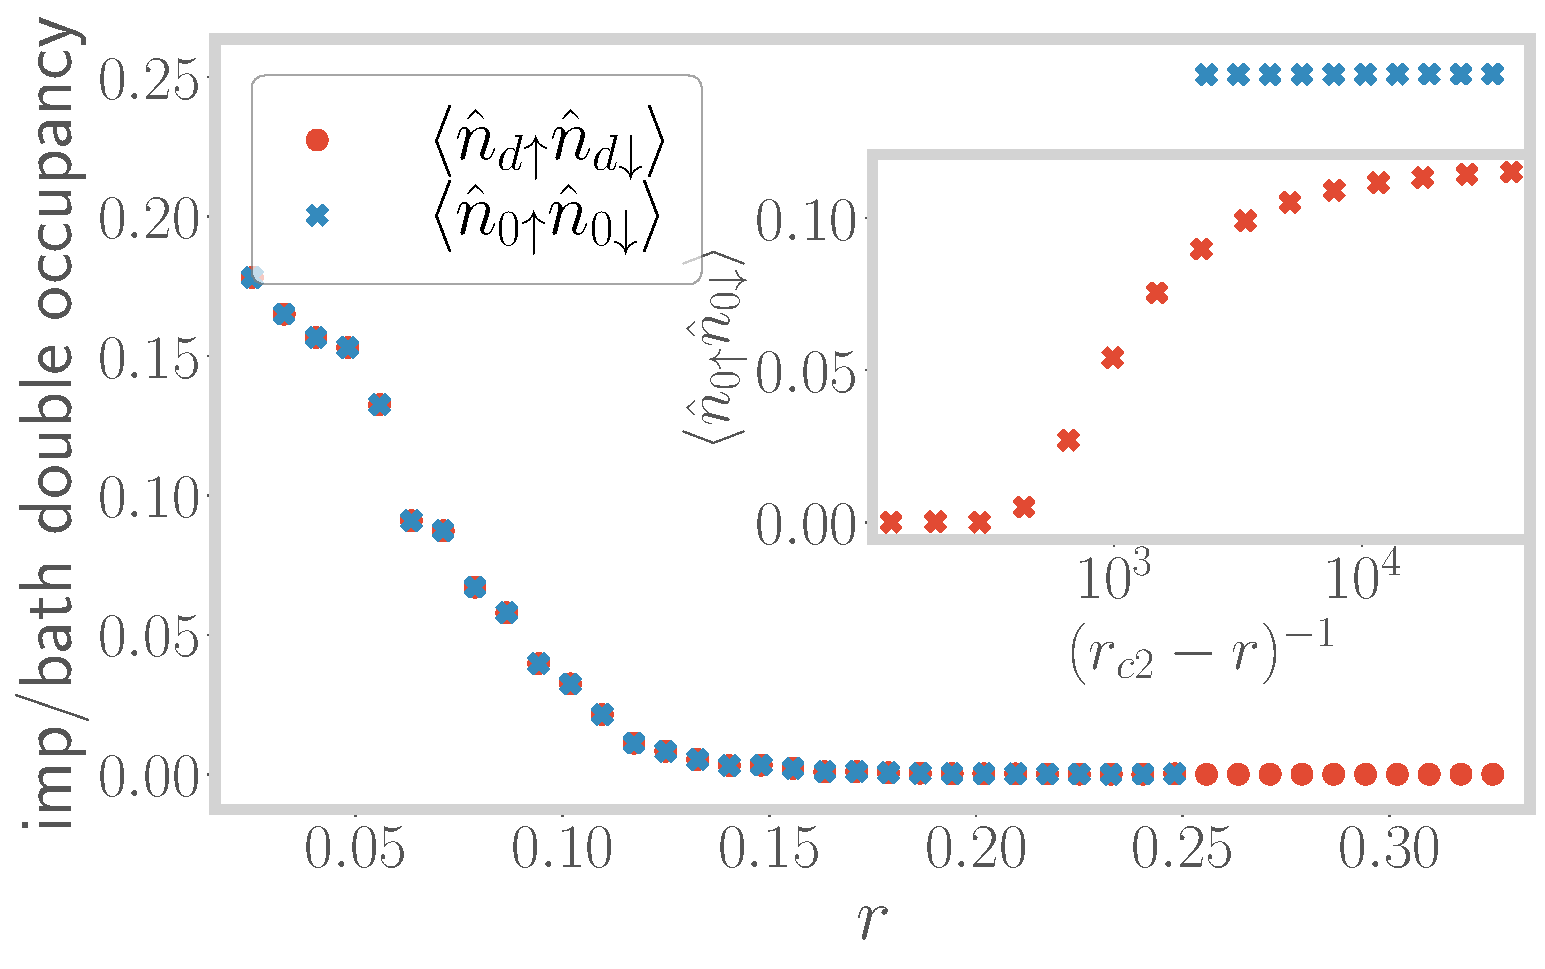
\includegraphics[width=0.48\textwidth]{doub_occ.pdf}
	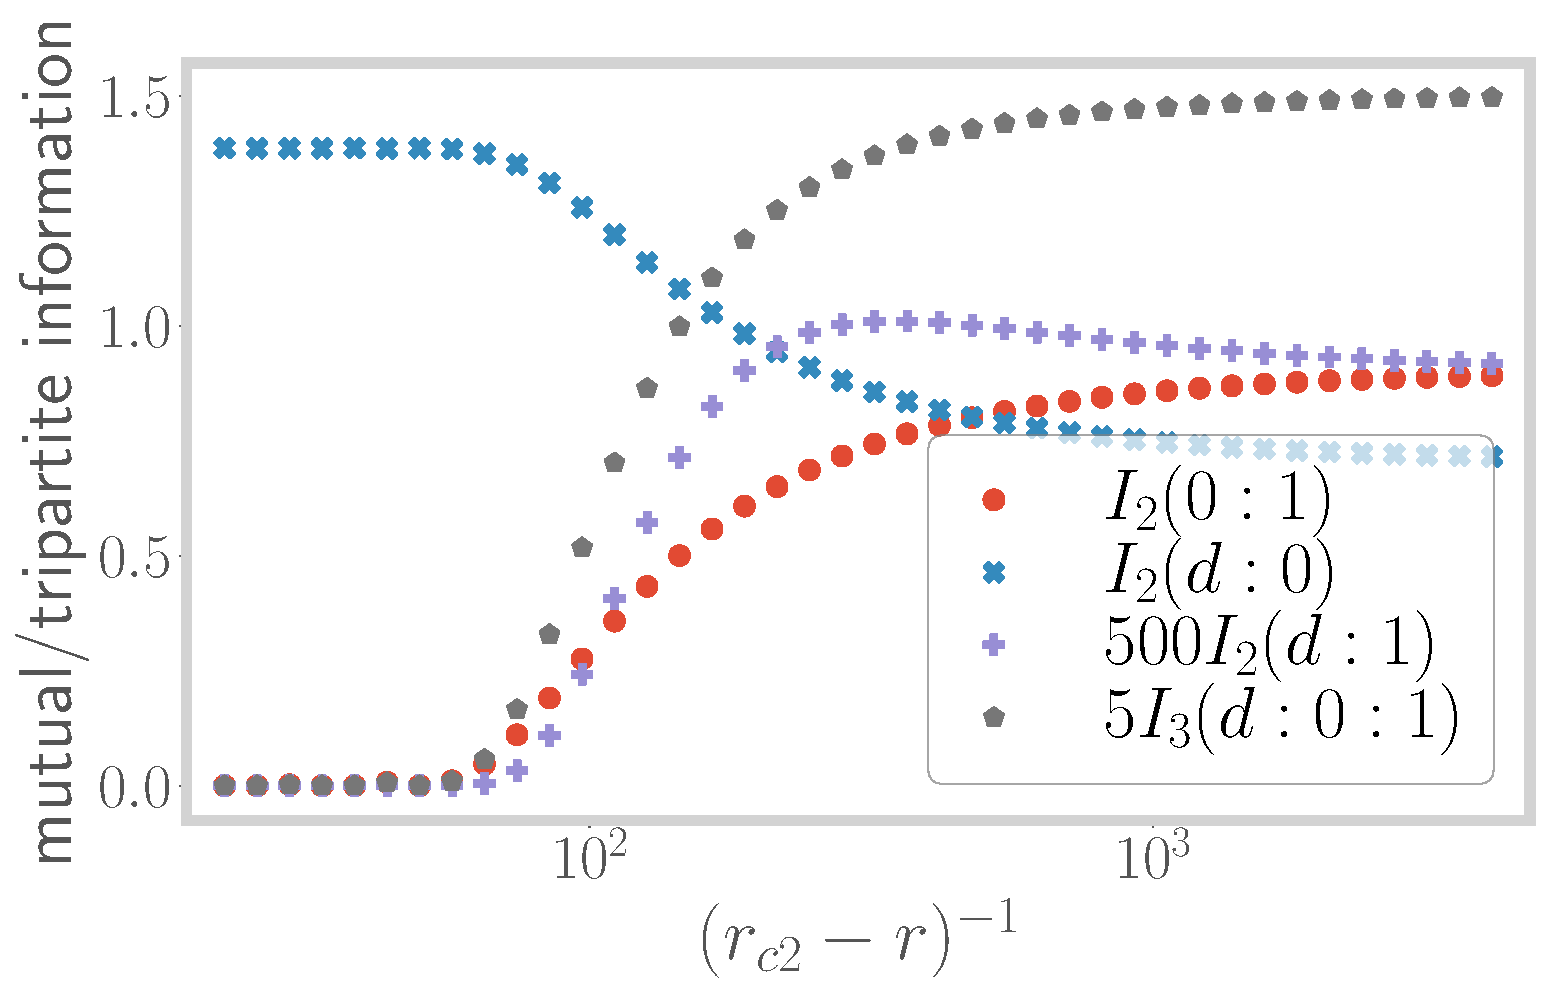
\includegraphics[width=0.48\textwidth]{rc2-mut-trip-info.pdf}
	\caption{Left: Evolution of the double occupancy of impurity (red) and zeroth sites (blue) ground-state double occupancy, with \(r\). Right: Evolution of various quantum information-theoretic measures, very close to the transition. }
	\label{fig1}
\end{figure}

\begin{figure}[htpb]
	\centering
	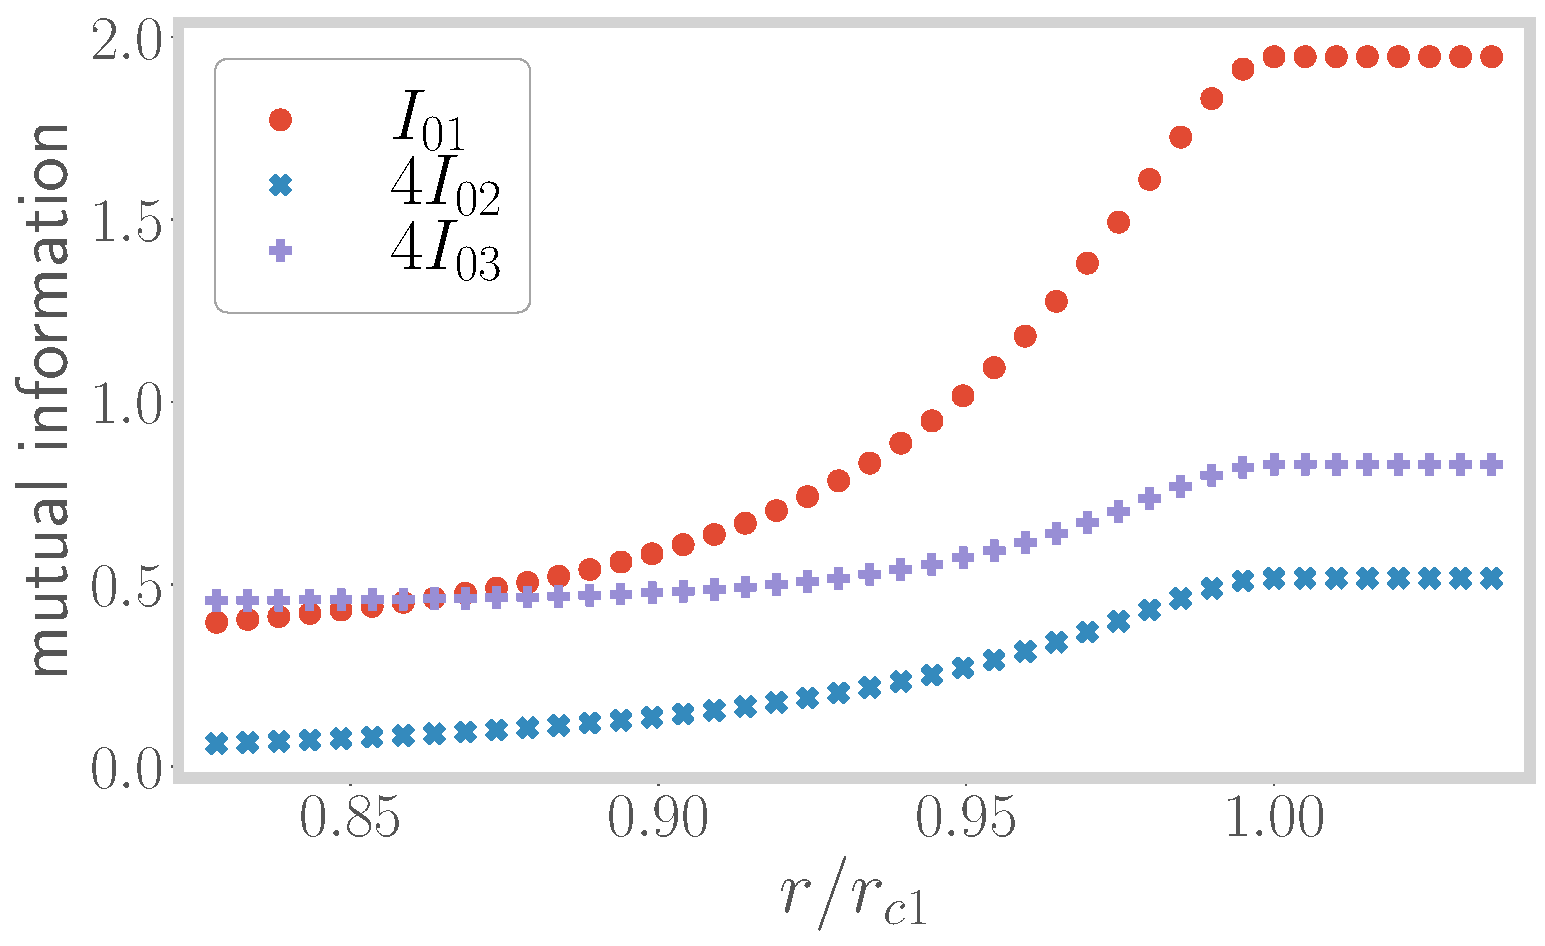
\includegraphics[width=0.48\textwidth]{Uc1-bath-mutinfo.pdf}
	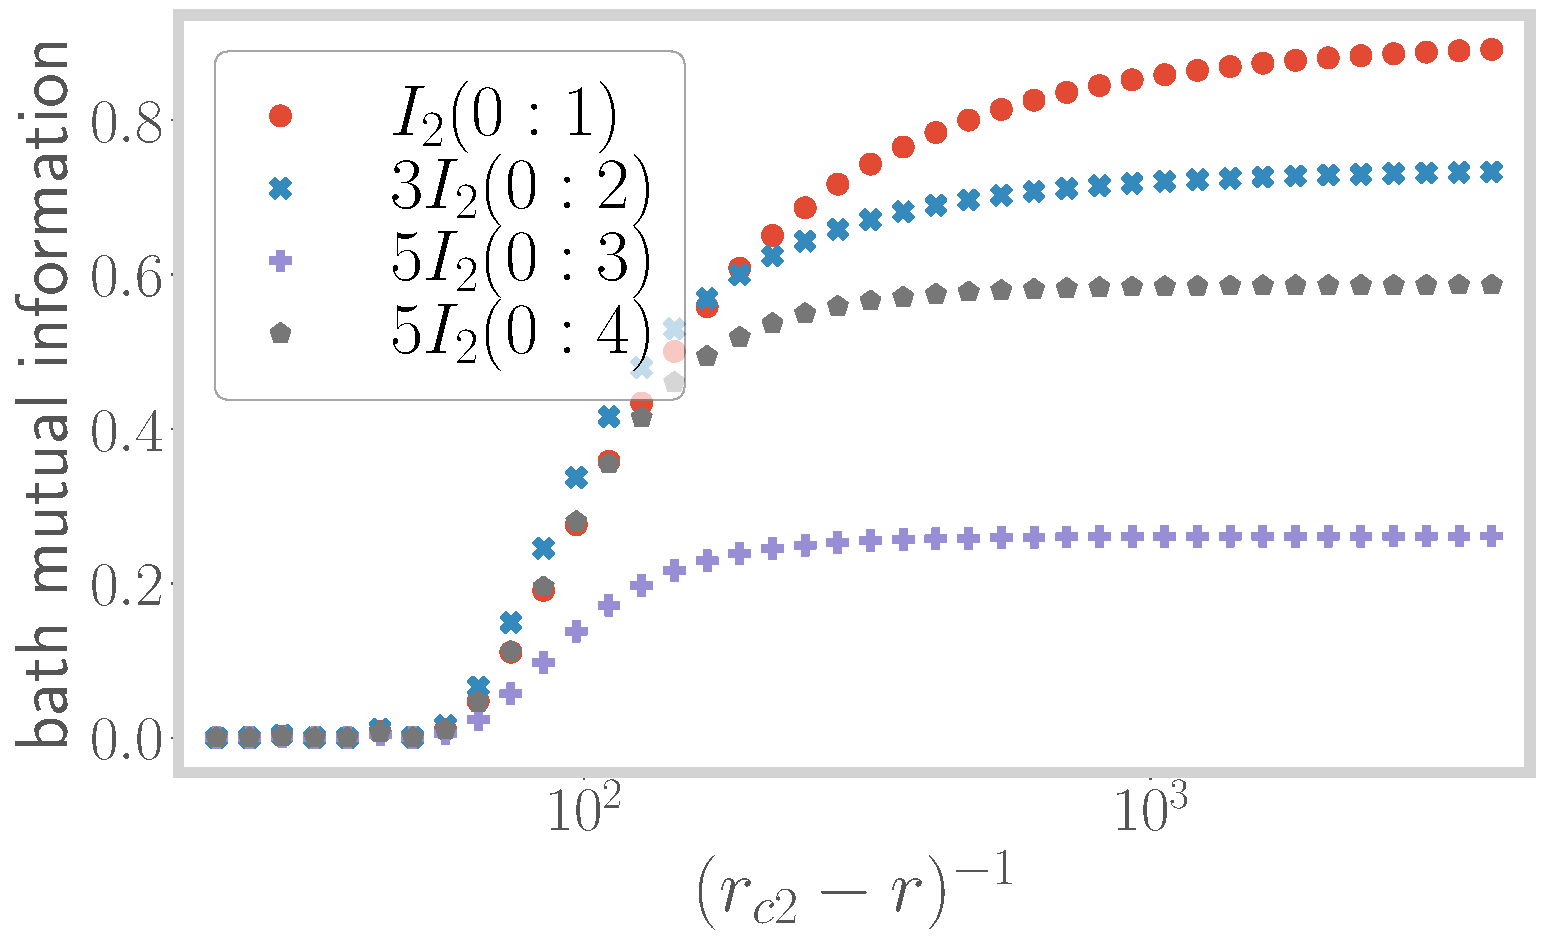
\includegraphics[width=0.48\textwidth]{rc2-mut-info-bath.pdf}
	\caption{Variation of intra-bath mutual information between zeroth site and sites 1, 2 and 3, near \(r_{c1}\) (left) and \(r_{c2}\) (right).}
	\label{fig2}
\end{figure}

\begin{figure}[htpb]
	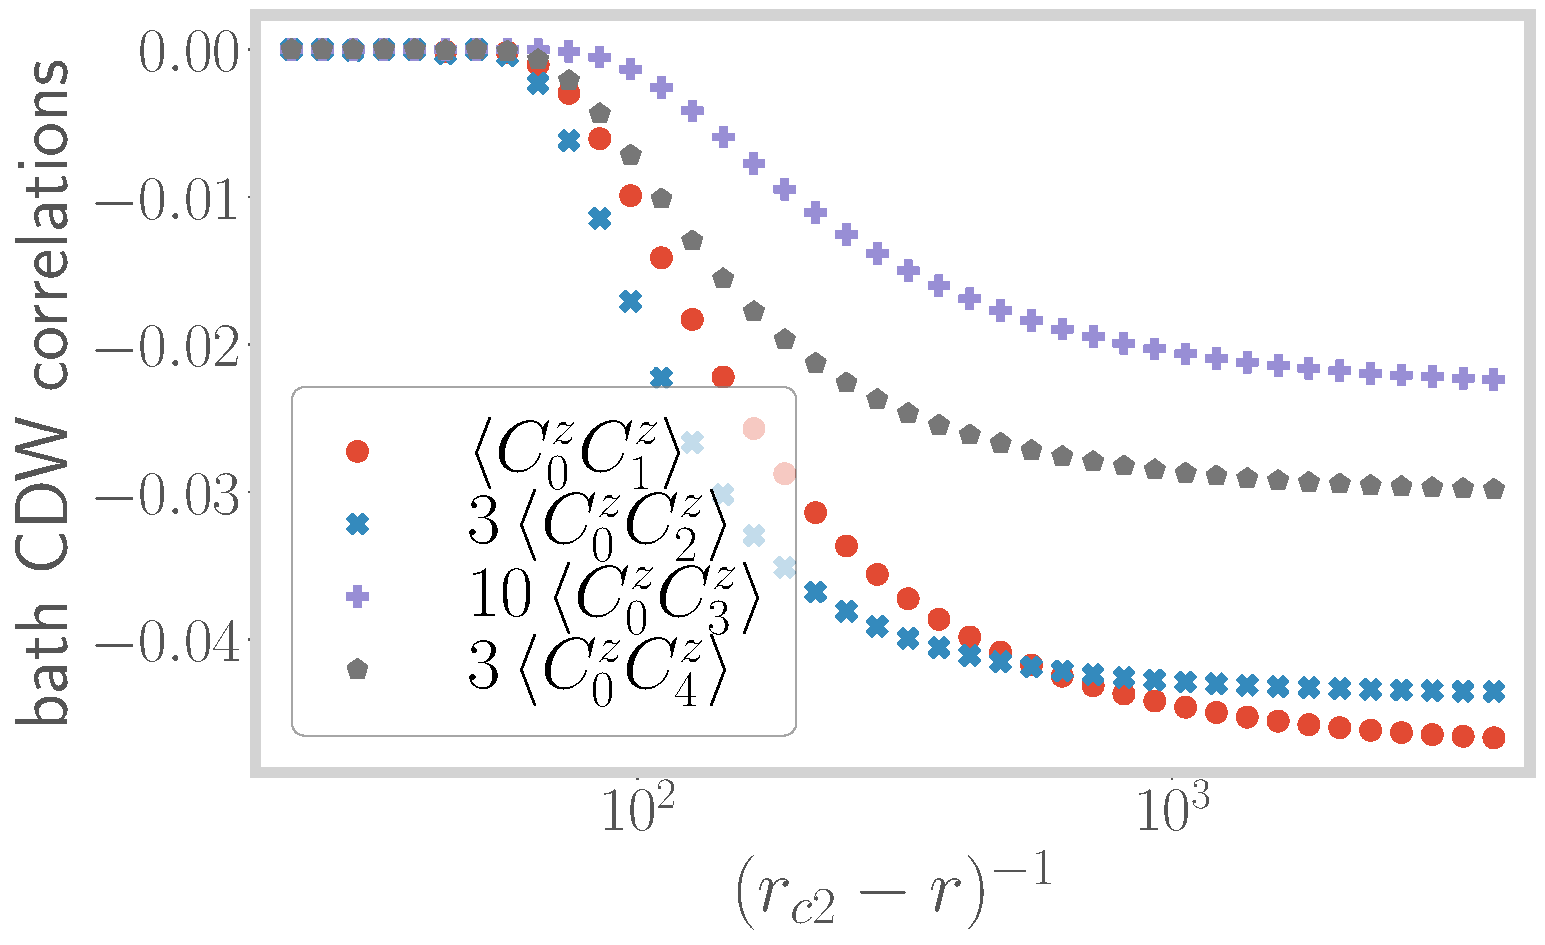
\includegraphics[width=0.48\textwidth]{rc2-charge-ising-corr-0i.pdf}
	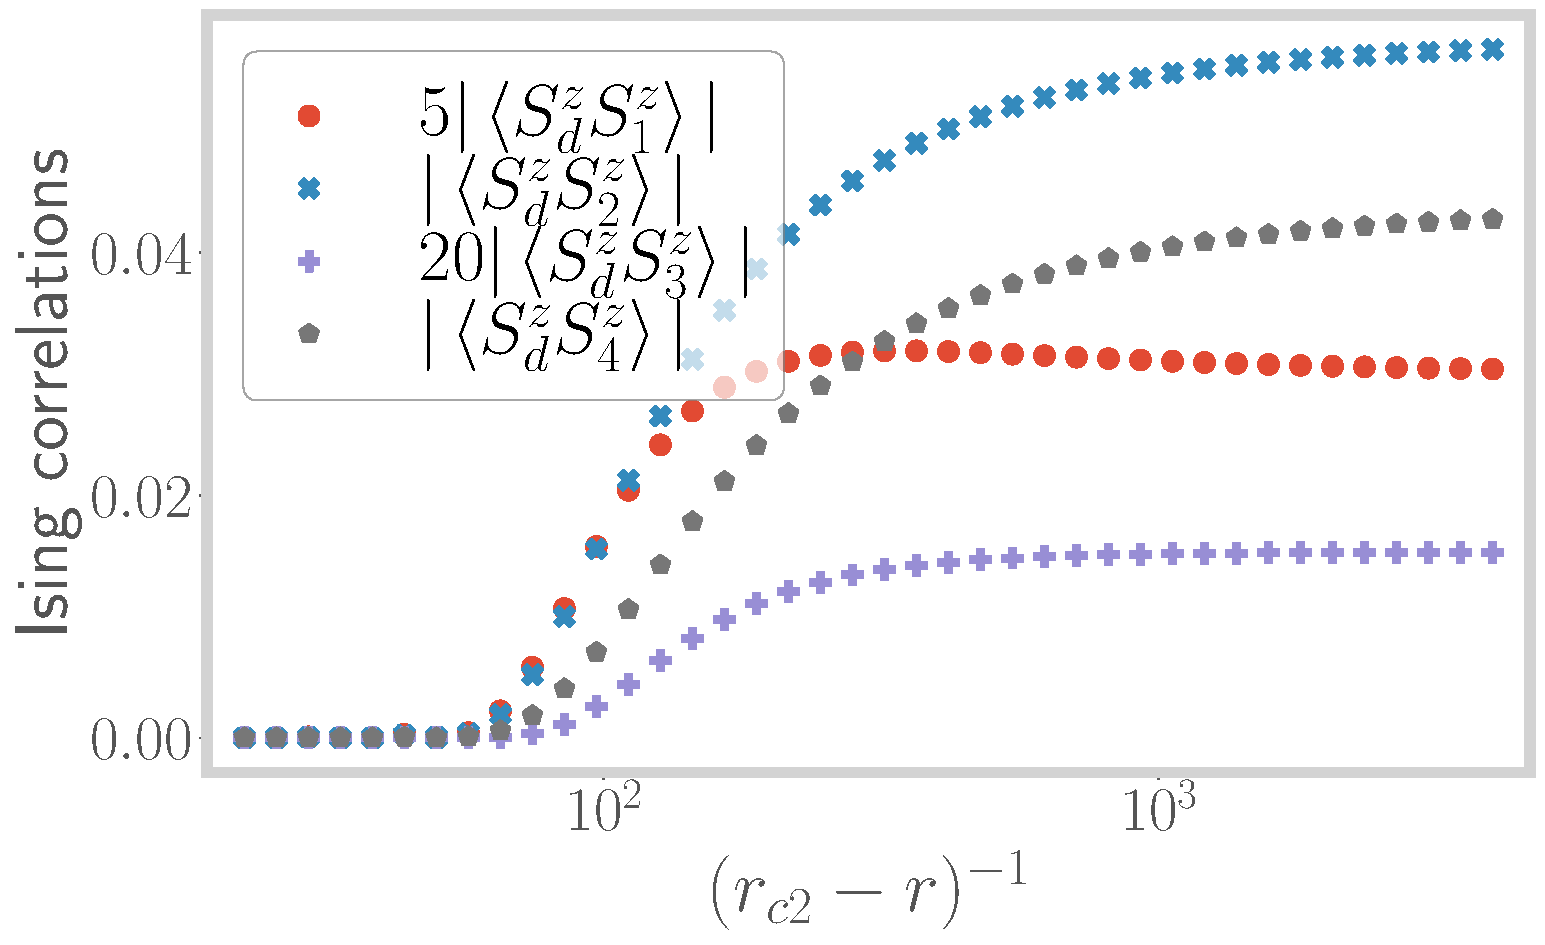
\includegraphics[width=0.48\textwidth]{rc2-spin-ising-corr-di.pdf}
	\caption{Left: Variation of charge isospin Ising correlations between the zeroth site and bath sites further down the chain. Right: Ising correlations between the impurity site and bath sites beyond the zeroth site. Both sets of correlations show an overall increase as \(r \to r_{c2}\).}
	\label{fig3}
\end{figure}

\section*{References}

\bibliography{esiam-manuscript}
\end{document}
